\documentclass[11pt]{article}
\usepackage[margin=1in]{geometry}
\usepackage{amsmath, amssymb, amsthm, bm}
\usepackage{mathtools}
\usepackage{enumitem}
\usepackage{hyperref}
\usepackage{natbib}
\usepackage{booktabs}
\usepackage{multirow}
\usepackage{graphicx}
\usepackage{xcolor}
\usepackage{algorithm}
\usepackage{algpseudocode}

%% theorem environments
\newtheorem{theorem}{Theorem}
\newtheorem{proposition}{Proposition}
\newtheorem{corollary}{Corollary}[theorem]
\newtheorem{remark}{Remark}
\theoremstyle{definition}
\newtheorem{definition}{Definition}

%% macros
\newcommand{\R}{\mathbb{R}}
\newcommand{\N}{\mathbb{N}}
\newcommand{\E}{\mathbb{E}}
\newcommand{\bI}{\mathbf{I}}
\newcommand{\Var}{\mathrm{Var}}
\newcommand{\calD}{\mathcal{D}}
\newcommand{\calU}{\mathcal{U}}
\newcommand{\calJ}{\mathcal{J}}
\newcommand{\calN}{\mathcal{N}}
\newcommand{\lam}{\lambda}
\newcommand{\Sig}{\Sigma}
\newcommand{\LSE}{\mathrm{LSE}}
\newcommand{\calQ}{\mathcal{Q}}
\newcommand{\calV}{\mathcal{V}}
\newcommand{\calL}{\mathcal{L}}
\newcommand{\calA}{\mathcal{A}}
\newcommand{\todo}[1]{\textcolor{red}{\textbf{[TODO: #1]}}}

\title{Semi-Supervised Generative Classification\\
       via a Weighted Unlabeled Likelihood}
\author{Aaron John Danielson}
\date{}

\begin{document}
\maketitle

%% ============================================================
\begin{abstract}
We study semi-supervised binary classification in settings where labeled positives
and negatives are scarce but unlabeled feature vectors are plentiful.
We propose a two-component Gaussian mixture model estimated by a weighted
likelihood that combines the fully observed class-conditional log-likelihoods
with a tunable multiple \(\lambda\) of the unlabeled marginal mixture
log-likelihood, fit by expectation-maximization with closed-form updates.
The central contribution is an analysis of \(\lambda\) as an object of study
in its own right.
We prove an implicit-function-theorem characterization of the pseudo-true
parameter path \(\theta^\star(\lambda)\): the derivative \(d\theta^\star/d\lambda\)
equals the negative inverse Hessian times the unlabeled score residual,
which is zero under correct specification and nonzero---and computable---under
misspecification.
This formula yields a computable pre-fitting score, the \emph{alignment
coefficient} \(\mathcal{A}(0)\), whose sign predicts whether adding unlabeled
data will improve or degrade the estimator.
We characterize \(\mathcal{A}(0)\) as a \emph{decision support tool} rather
than a universal oracle: in the small-labeled-data regime
(the setting where semi-supervised learning is most consequential),
the binary use/discard decision based on the sign of \(\hat{\mathcal{A}}(0)\)
achieves 65--72\% accuracy with mean regret below 0.01 AUROC;
as labeled data grow, regret collapses below 0.001 regardless of the decision,
making the diagnostic most useful exactly when the decision matters most.
We further propose a confidence-weighted generalization \(\lambda(x)\) that
downweights ambiguous unlabeled points, prove a component-wise score-attenuation
property under a directional coherence condition, and implement it via an
MM surrogate with closed-form updates at each iteration.
Theorem~\ref{thm:path} additionally yields a gradient-based procedure for
\emph{learning} \(\lambda\) from a validation set, reducing \(\lambda\)-selection
to gradient ascent rather than grid search.
Simulations across four estimation regimes---unsupervised mixture, small-sample
supervised, global-\(\lambda\) semi-supervised, and confidence-weighted
semi-supervised---demonstrate progressive improvement in parameter recovery
and classification accuracy.
We further validate on five UCI benchmarks, showing that the score-residual
norm \(\|\hat{g}_0\|\) correctly identifies datasets where the Gaussian
assumption fails and semi-supervised learning is inadvisable.
An open-source Python implementation is available as the
\texttt{semi\_supervised\_em} package.
\end{abstract}

%% ============================================================
\section{Introduction}
\label{sec:intro}

Many applied classification problems share the same structural constraint:
labels are expensive but features are abundant.
A clinician can pull millions of electronic records but has time to adjudicate
only hundreds.
An insurer can process millions of claim events but has expert labels for a
small fraction of matches.
A sports analyst can observe thousands of player-possession observations
but can verify only a handful by hand.
In each case, the practitioner faces a partially labeled problem: a small
labeled set that anchors the decision boundary and a large unlabeled corpus
whose structure may sharpen or distort it.

Purely supervised models discard the unlabeled structure entirely and face
high-variance estimation when labels are few.
Fully unsupervised mixture fitting ignores the labeled anchors and can converge
to components that are uninformative for the classification task.
Semi-supervised approaches attempt to exploit both, but the literature offers
a wide spectrum of methods---from generative likelihood-based models at one
end to discriminative consistency regularization at the other---with different
assumptions about how unlabeled data relate to the task.

This paper proposes and analyzes a simple, transparent semi-supervised
generative classifier.
We model the class-conditional distributions as multivariate Gaussians and
estimate parameters by maximizing a \emph{weighted} log-likelihood,
\begin{equation}
\calJ_\lam(\theta)
= \underbrace{\ell_{\mathrm{sup}}(\theta)}_{\text{supervised}}
+ \lam\,\underbrace{\ell_{\mathrm{unl}}(\theta)}_{\text{unlabeled mixture}},
\label{eq:intro-objective}
\end{equation}
where \(\lam>0\) is a scalar weight that controls how much the unlabeled
corpus influences the fit.
This objective is maximized by expectation-maximization (EM), which yields
closed-form parameter updates in each iteration.

The weight \(\lam\) is not merely a tuning nuisance; it is the conceptual
spine of the paper.
Increasing \(\lam\) from zero continuously deforms the estimator from the
purely supervised maximum likelihood estimator (MLE) toward an unlabeled-mixture-dominated fit.
Each unit of \(\lam\) can be interpreted as contributing an
\emph{effective} unlabeled sample budget of \(\lam N_u\) additional soft
observations, partitioned across classes according to the current
responsibilities.
This effective-sample-size interpretation makes \(\lam\) actionable:
a practitioner can set it by asking how many additional pseudo-labeled
examples the unlabeled corpus should count for, rather than treating it
as an opaque regularization coefficient.

Under model misspecification---when the true class-conditional distributions
are not Gaussian---the estimator converges to a \(\lam\)-dependent
pseudo-true parameter that can differ from the supervised pseudo-true
parameter and may move the decision boundary in an unhelpful direction.
We characterize this dependence and show that it motivates treating
\(\lam\) as a diagnostic as well as a tuning parameter: if increasing
\(\lam\) degrades labeled-set performance, the unlabeled structure is
inconsistent with the Gaussian model and caution is warranted.

\paragraph{Motivating application.}
Our primary application is note-to-claimant matching at an insurance
company.
Each claim generates a set of notes (free text or structured records),
each of which must be matched to one of several candidate claimants
within the claim.
Expert labels are available for a small fraction of note-claimant pairs,
while a much larger corpus of feature-described pairs has no label.
At inference time, the model produces a score $s(x) = \Pr(z=1\mid x;\hat\theta)$
for each candidate pair, and scores are renormalized within each claim
to enforce competition among candidates.
This within-claim renormalization converts global posteriors into a
proper ranking over candidates.

\paragraph{Contributions.}
\begin{enumerate}[leftmargin=1.5em,label=\arabic*.]
\item A weighted semi-supervised Gaussian mixture objective with unlabeled
      weight \(\lam\) as the interpretable control parameter, fit by EM
      with closed-form updates (Section~\ref{sec:method}).
\item A formal effective-sample-size interpretation of \(\lam\):
      the fixed-point estimator is a weighted average of labeled
      sufficient statistics and responsibility-weighted unlabeled
      sufficient statistics (Proposition~\ref{prop:ess}).
\item An implicit-function-theorem theorem (Theorem~\ref{thm:path})
      giving the exact derivative \(d\theta^\star(\lam)/d\lam\)
      in terms of the unlabeled score residual at the supervised pseudo-true
      parameter---zero under correct specification, nonzero and computable
      under misspecification---plus a sample diagnostic \(\hat g_0\)
      that can be evaluated before fitting.
\item A confidence-weighted generalization \(\lambda(x_j) = \lam\cdot
      (\max_g\gamma_j^{(g)})^\alpha\) implemented via an MM surrogate
      with closed-form updates, and a proven component-wise score-attenuation
      property under a directional coherence condition
      (Proposition~\ref{prop:conf-safety}).
\item A gradient-based procedure for \emph{learning} \(\lam\) from data
      (Section~\ref{sec:learn-lam}): the IFT derivative~\eqref{eq:path-derivative}
      yields a closed-form alignment coefficient \(\calA(0)\) whose sign
      provides a decision-support diagnostic for whether to use unlabeled data.
      In the small-label regime, the binary decision \(D=\mathbf{1}[\hat\calA(0)>0]\)
      achieves 65--72\% accuracy with mean regret below 0.01 AUROC;
      the diagnostic is most reliable precisely when the unlabeled contribution
      is largest and the decision is most consequential.
\item Simulation evidence across four regimes
      (unsupervised, supervised, global-\(\lam\), confidence-weighted)
      on parameter recovery, classification accuracy, calibration,
      and robustness to misspecification.
\item Empirical validation on five UCI binary classification benchmarks,
      showing that the score-residual norm \(\|\hat g_0\|\) correctly identifies
      the near-Gaussian datasets (Banknote, Breast Cancer) where the diagnostic
      achieves 65--70\% accuracy from the non-Gaussian ones (Ionosphere, Sonar,
      Spambase) where it falls to 40--50\%.
\item An open-source Python package, \texttt{semi\_supervised\_em},
      with a scikit-learn-compatible API.
\end{enumerate}

\paragraph{The unifying thread.}
The score residual \(\hat g_0\)---the gradient of the unlabeled log-likelihood
evaluated at the supervised MLE---is the paper's load-bearing object,
but its two roles must be carefully distinguished.

\emph{Its norm} \(\|\hat g_0\|\) is a pre-fitting indicator of
\emph{magnitude of mismatch}: a large norm means the unlabeled corpus is
structurally inconsistent with the Gaussian model and that the parameter
path will move rapidly as \(\lam\) grows.
It does not by itself say whether that movement helps or hurts.

\emph{Its direction}, via the alignment coefficient
\(\calA(0) = -\nabla_\theta\ell_{\calV}(\hat\theta(0))^\top
\hat H(0)^{-1}\hat g_0\),
is the \emph{directional} diagnostic:
if \(\calA(0)>0\), the unlabeled data pull the estimator toward the
validation optimum; if \(\calA(0)<0\), they pull it away.
Gradient ascent on \(\lam\) increases validation likelihood if and only
if \(\calA(\lam)>0\).

The single formula \(d\theta^\star/d\lam = -H^{-1}g_0\) thus serves
simultaneously as magnitude certificate (via \(\|H^{-1}g_0\|\)),
directional diagnostic (via its inner product with the validation gradient),
and optimization oracle---computed in one Hessian solve at essentially no
additional cost beyond the supervised fit.
Corollary~\ref{cor:second-order} further shows that \(\calA(0)\) predicts
the first-order change in validation likelihood, with the second-order term
explaining why the prediction degrades at larger \(\lam\).

\paragraph{Paper outline.}
Section~\ref{sec:related} reviews related work.
Section~\ref{sec:method} defines the model and EM algorithm.
Section~\ref{sec:theory} develops the theoretical analysis.
Sections~\ref{sec:simulations} and~\ref{sec:empirical} present simulation
and empirical results.
Section~\ref{sec:discussion} discusses scope and limitations.


%% ============================================================
\section{Related Work}
\label{sec:related}

\subsection{Semi-Supervised Learning}

Semi-supervised learning has a long history; comprehensive surveys include
\citet{zhu2005semi} and \citet{chapelle2006semi}.
Methods divide broadly into generative and discriminative families.
Generative semi-supervised methods learn a joint model of features and
labels and use unlabeled examples to improve the marginal feature distribution estimate.
The classical example is EM for Gaussian mixtures with partially
observed class labels \citep{dempster1977maximum, ghahramani1994supervised}.
Discriminative methods---including consistency regularization
\citep{laine2016temporal, miyato2018virtual}, pseudo-labeling
\citep{lee2013pseudo}, and self-training \citep{scudder1965probability}---add
unlabeled data through surrogate losses or teacher-student loops
without committing to a generative model.

Our method is generative and likelihood-based, placing it closest to the
tradition of \citet{ghahramani1994supervised} and \citet{nigam2000text}.
\citet{nigam2000text} use a related downweighting of unlabeled data in
naive Bayes text classification; they note empirically that reducing the
unlabeled weight can improve performance when the generative assumptions
are violated, but do not derive the effective-sample-size interpretation
or the pseudo-true parameter path.

\subsection{Gaussian Mixture Models, Weighting, and Misspecification}

Two-component Gaussian mixture models are a canonical probabilistic
classification tool \citep{fraley2002model, mcnicholas2016mixture}.
The maximum likelihood problem for partially labeled Gaussian mixtures
has been studied by \citet{ganesalingam1978classification} and
\citet{o1978normal}, and \citet{banfield1993model} develop model-based
clustering via EM for the fully unlabeled case.

\paragraph{Closest method-level comparator.}
\citet{huang2009semi} study semi-supervised Gaussian mixture models
for phonetic classification with an explicit relative weighting between
labeled and unlabeled log-likelihoods, including empirical analysis of
critical weight values and how they vary with labeled sample size.
Our paper is complementary: we develop a focused analytical treatment
of the same weighting parameter in the simplest Gaussian generative
binary classifier, contributing (i) the implicit-function-theorem
characterization of the pseudo-true parameter path, (ii) the closed-form
score-residual diagnostic \(\hat g_0\), and (iii) the confidence-weighted
extension with its provable damage bound---none of which appear in
\citet{huang2009semi}.

\paragraph{Closest conceptual comparator.}
\citet{ji2009semisupervised} study semi-supervised hidden Markov models
via a homotopy approach in which a parameter continuously interpolates
between supervised (\(\lam=0\)) and unsupervised (\(\lam=1\)) objectives,
and discuss performance degradation under misspecification.
Our Theorem~\ref{thm:path} provides an estimator-level companion to that
interpolation idea: rather than tracking the optimization path numerically,
we give a formula for how the fixed-point target moves as \(\lam\) varies.

\paragraph{Misspecification.}
\citet{cozman2002unlabeled} show rigorously that unlabeled data can
\emph{decrease} the accuracy of generative classifiers under model
misspecification.
Their result is qualitative; our Theorem~\ref{thm:path} provides a
quantitative companion, giving the rate and direction of estimand damage
as a function of \(\lam\) via the score residual \(g_0\).
The confidence-weighted \(\lam(x)\) in Section~\ref{sec:conf-weighted}
is a direct algorithmic response: under a directional coherence condition
it attenuates each coordinate of the score residual, reducing per-coordinate
misspecification exposure (Proposition~\ref{prop:conf-safety}).

\subsection{Positive-Unlabeled and Weakly Supervised Learning}

Positive-unlabeled (PU) learning \citep{liu2002partially, elkan2008learning}
considers a setting where only positive labels are observed and the
negative class must be inferred from the unlabeled pool.
Our setting is distinct: we observe labeled positives \emph{and} labeled
negatives, so the supervised component anchors both class-conditional
distributions.
When labeled negatives are sparse, our method naturally degrades gracefully
because the unlabeled likelihood can inform the negative component;
this is a point of contact with PU learning, but the formal setup differs.

Weakly supervised methods \citep{zhou2018brief, ratner2017snorkel} use
programmatic or noisy labels rather than unlabeled examples per se.
Our unlabeled examples carry no label information at all; they enter
only through the generative model's marginal likelihood.

\subsection{Entity Matching and Candidate Ranking}

The notes-to-claimants matching problem belongs to the entity matching
and record linkage literature \citep{fellegi1969theory, christophides2020overview}.
Standard approaches include rule-based blocking, string-similarity
classifiers, and learning-to-rank methods.
Semi-supervised generative models have been applied to record linkage
by \citet{larsen2001iterative}, who use EM on the Fellegi-Sunter model.
Our method differs in operating on arbitrary numeric feature vectors
rather than agreement patterns, and in explicitly modeling within-claim
competition through post-hoc score renormalization.


%% ============================================================
\section{Method}
\label{sec:method}

\subsection{Problem Setting and Notation}

We observe feature vectors \(x\in\R^m\).
Data are partitioned into labeled positives (\(z=1\)), labeled negatives (\(z=0\)),
and unlabeled examples:
\[
\calD_1=\{x_i^{(1)}\}_{i=1}^{N_1},\qquad
\calD_0=\{x_i^{(0)}\}_{i=1}^{N_0},\qquad
\calU=\{x_j^{(u)}\}_{j=1}^{N_u}.
\]
Let \(N_{\mathrm{obs}}=N_0+N_1\).
We assume all observations are drawn from a two-component Gaussian mixture,
\[
x \;\sim\; \pi\,\calN(\mu_1,\Sig_1) + (1-\pi)\,\calN(\mu_0,\Sig_0),
\]
and that the labeled sets are draws conditional on their respective class
labels.
We write parameters collectively as
\(\theta=(\pi,\mu_1,\mu_0,\Sig_1,\Sig_0)\), where for \(g\in\{0,1\}\):
\[
x\mid z=g \sim \calN(\mu_g,\Sig_g),
\qquad \Pr(z=1)=\pi,\ \Pr(z=0)=1-\pi.
\]
The multivariate Gaussian density is
\[
\calN(x\mid \mu,\Sig)=\frac{1}{(2\pi)^{m/2}|\Sig|^{1/2}}
\exp\!\Big(-\tfrac{1}{2}(x-\mu)^\top\Sig^{-1}(x-\mu)\Big).
\]

\subsection{Weighted Semi-Supervised Objective}

We maximize a \emph{weighted} log-likelihood combining labeled
and unlabeled examples with unlabeled weight \(\lam>0\):
\begin{align}
\calJ_\lam(\theta)
&= \sum_{i=1}^{N_1}\log\!\Big[\pi\,\calN(x_i^{(1)}\mid \mu_1,\Sig_1)\Big]
 + \sum_{i=1}^{N_0}\log\!\Big[(1-\pi)\,\calN(x_i^{(0)}\mid \mu_0,\Sig_0)\Big] \nonumber\\
&\quad + \lam \sum_{j=1}^{N_u}\log\!\Big(
\pi\,\calN(x_j^{(u)}\mid \mu_1,\Sig_1) + (1-\pi)\,\calN(x_j^{(u)}\mid \mu_0,\Sig_0)
\Big). \label{eq:weighted-ll}
\end{align}
The labeled terms use the \emph{joint} class likelihood
\(p_\theta(x,z)\), not the class-conditional \(p_\theta(x\mid z)\),
so \(\pi\) is identified by the labeled class counts as well as by the
unlabeled responsibilities.
When \(\lam\!\to\!0\) we recover the purely supervised joint MLE;
when \(\lam\) is large, the unlabeled mixture log-likelihood dominates.

\subsection{EM Algorithm}

Direct maximization of \(\calJ_\lam\) is intractable because of the
log-sum in the unlabeled term.
We instead apply the EM algorithm, treating the latent class labels
\(z_j^{(u)}\in\{0,1\}\) of unlabeled examples as missing data.

Define responsibilities
\[
\gamma_j \;\coloneqq\; \Pr(z^{(u)}_j=1\mid x_j^{(u)};\theta)
= \frac{\pi\,\calN(x_j^{(u)}\mid \mu_1,\Sig_1)}
{\pi\,\calN(x_j^{(u)}\mid \mu_1,\Sig_1) + (1-\pi)\,\calN(x_j^{(u)}\mid \mu_0,\Sig_0)}.
\]
Define the \emph{soft counts}
\[
\widetilde{N}_1 = N_1 + \lam \sum_{j=1}^{N_u}\gamma_j,\qquad
\widetilde{N}_0 = N_0 + \lam \sum_{j=1}^{N_u}(1-\gamma_j),\qquad
\widetilde{N} = N_{\mathrm{obs}} + \lam N_u.
\]

\paragraph{E-step.}
Given \(\theta^{(t)}\), update responsibilities \(\gamma_j\) for all unlabeled
points.
Compute in log-space for numerical stability:
\[
\log r_{1j}=\log \pi + \log \calN(x_j^{(u)}\mid \mu_1,\Sig_1),\qquad
\log r_{0j}=\log (1-\pi) + \log \calN(x_j^{(u)}\mid \mu_0,\Sig_0),
\]
\[
\gamma_j = \exp\big(\log r_{1j} - \LSE(\log r_{1j},\log r_{0j})\big),
\]
where \(\LSE(a,b)=\max(a,b)+\log(e^{a-\max}+e^{b-\max})\).

\paragraph{M-step.}
Maximize the expected weighted complete-data log-likelihood to obtain
closed-form updates:
\begin{align}
\pi^{\text{new}} &= \frac{\widetilde{N}_1}{\widetilde{N}}, \label{eq:pi-update}\\[4pt]
\mu_1^{\text{new}} &= \frac{{\displaystyle\sum_{x\in \calD_1}} x
  + \lam \sum_{j=1}^{N_u} \gamma_j x_j^{(u)}}{\widetilde{N}_1},
\qquad
\mu_0^{\text{new}} = \frac{{\displaystyle\sum_{x\in \calD_0}} x
  + \lam \sum_{j=1}^{N_u} (1-\gamma_j) x_j^{(u)}}{\widetilde{N}_0},
\label{eq:mu-update}\\[4pt]
\Sig_1^{\text{new}} &=
\frac{
{\displaystyle\sum_{x\in \calD_1}} (x-\mu_1^{\text{new}})(x-\mu_1^{\text{new}})^\top
+ \lam \sum_{j=1}^{N_u} \gamma_j (x_j^{(u)}-\mu_1^{\text{new}})(x_j^{(u)}-\mu_1^{\text{new}})^\top
}{\widetilde{N}_1} + \epsilon\bI, \label{eq:sig1-update}\\[4pt]
\Sig_0^{\text{new}} &=
\frac{
{\displaystyle\sum_{x\in \calD_0}} (x-\mu_0^{\text{new}})(x-\mu_0^{\text{new}})^\top
+ \lam \sum_{j=1}^{N_u} (1-\gamma_j) (x_j^{(u)}-\mu_0^{\text{new}})(x_j^{(u)}-\mu_0^{\text{new}})^\top
}{\widetilde{N}_0} + \epsilon\bI,
\label{eq:sig0-update}
\end{align}
where \(\epsilon>0\) is a small ridge constant that enforces positive definiteness.

\paragraph{Derivation sketch.}
Form the expected weighted complete-data log-likelihood
\(\calQ_\lam(\theta;\theta^{(t)}) = \E[\log p(X,Z;\theta)\mid X;\theta^{(t)}]\)
where unlabeled contributions are weighted by \(\lam\), take partial derivatives
with respect to each parameter, set to zero, and solve.
Equations~\eqref{eq:pi-update}--\eqref{eq:sig0-update} are the unique
maximizers under standard regularity (positive-definite covariances).

\paragraph{Convergence and initialization.}
Repeat E/M steps until
\[
\max\!\Big\{\|\mu_1^{\text{new}}-\mu_1\|_\infty, \|\mu_0^{\text{new}}-\mu_0\|_\infty,
\|\Sig_1^{\text{new}}-\Sig_1\|_\infty, \|\Sig_0^{\text{new}}-\Sig_0\|_\infty,
|\pi^{\text{new}}-\pi|\Big\}<\varepsilon.
\]
A robust warm start uses the supervised MLEs:
\[
\mu_g^{(0)}=\frac{1}{N_g}\sum_{x\in\calD_g}x,\qquad
\Sig_g^{(0)}=\frac{1}{N_g}\sum_{x\in\calD_g}(x-\mu_g^{(0)})(x-\mu_g^{(0)})^\top + \epsilon\bI,
\qquad
\pi^{(0)}=\frac{N_1}{N_{\mathrm{obs}}}.
\]
Unlabeled responsibilities are initialized as \(\gamma_j^{(0)}=\pi^{(0)}\).
This ensures that EM begins from a configuration that is already consistent
with the labeled data, reducing sensitivity to initialization and accelerating
convergence.

\begin{algorithm}[t]
\caption{Weighted Semi-Supervised EM}
\label{alg:ssem}
\begin{algorithmic}[1]
\Require $\calD_1$, $\calD_0$, $\calU$, weight $\lam>0$, tolerance $\varepsilon$, ridge $\epsilon$
\State Initialize $\mu_g^{(0)},\Sig_g^{(0)},\pi^{(0)}$ from supervised MLEs;
       set $\gamma_j^{(0)} = \pi^{(0)}$
\Repeat
  \State \textbf{E-step:} Compute $\gamma_j$ via log-sum-exp for all $j$
  \State \textbf{M-step:} Update $\pi,\mu_g,\Sig_g$ via
         \eqref{eq:pi-update}--\eqref{eq:sig0-update}
\Until{max parameter change $< \varepsilon$}
\Return $\hat\theta = (\hat\pi, \hat\mu_1, \hat\mu_0, \hat\Sig_1, \hat\Sig_0)$
\end{algorithmic}
\end{algorithm}

\subsection{Confidence-Weighted Unlabeled Likelihood}
\label{sec:conf-weighted}

The scalar \(\lam\) treats all unlabeled points equally.
We propose a point-wise generalization:
\begin{equation}
\calJ_{\lam,\alpha}(\theta)
= \ell_{\mathrm{sup}}(\theta)
  + \lam\sum_{j\in\calU}
    w_j^{(\alpha)}(\theta)\,
    \log p_\theta(x_j^{(u)}),
\label{eq:conf-objective}
\end{equation}
where the confidence weight of unlabeled point \(j\) is
\begin{equation}
w_j^{(\alpha)}(\theta)
= \Bigl(\max_{g\in\{0,1\}}\gamma_j^{(g)}(\theta)\Bigr)^\alpha,
\qquad \alpha\geq 0,
\label{eq:conf-weight}
\end{equation}
with \(\gamma_j^{(1)}=\gamma_j\) and \(\gamma_j^{(0)}=1-\gamma_j\).
At \(\alpha=0\) we recover the uniform-\(\lam\) objective.
As \(\alpha\to\infty\) only the most confidently classified unlabeled points contribute.
For a point classified with certainty, \(w_j^{(\alpha)}=1\); for a
maximally ambiguous point (\(\gamma_j=0.5\)), \(w_j^{(\alpha)}=2^{-\alpha}\).

\paragraph{Algorithm under confidence weighting (MM surrogate).}
Because \(w_j^{(\alpha)}(\theta)\) depends on \(\theta\), the objective
\eqref{eq:conf-objective} is \emph{not} a standard weighted log-likelihood
with fixed weights, and direct EM does not apply.
We instead treat this as a majorization-minimization (MM) procedure:
at iteration \(t\), \emph{freeze} the confidence weights at the current parameter,
\[
\tilde w_j^{(t)} \;=\; \lam\,w_j^{(\alpha)}(\theta^{(t)}),
\]
and maximize the resulting surrogate objective—a weighted mixture
log-likelihood with \emph{fixed} point-weights \(\tilde w_j^{(t)}\).
The E-step computes responsibilities \(\gamma_j\) at \(\theta^{(t)}\) as before.
The M-step soft counts become
\[
\widetilde N_1^{(\alpha)} = N_1 + \sum_j \tilde w_j^{(t)}\,\gamma_j,
\qquad
\widetilde N_0^{(\alpha)} = N_0 + \sum_j \tilde w_j^{(t)}\,(1-\gamma_j),
\qquad
\widetilde N^{(\alpha)} = N_{\mathrm{obs}} + \sum_j \tilde w_j^{(t)},
\]
and update equations~\eqref{eq:pi-update}--\eqref{eq:sig0-update} carry
through with \(\lam\) replaced by \(\tilde w_j^{(t)}\) for point \(j\).
All M-step updates are closed-form for the surrogate.
Proposition~\ref{prop:em} (monotonicity) applies to each surrogate step
but \emph{not} globally across iterations, because the surrogate changes at
each step when the weights are refreshed.
In practice the algorithm converges reliably; we do not claim that it
increases the true objective \eqref{eq:conf-objective} at every step.

\subsection{Numerical Considerations}

\begin{itemize}[leftmargin=1.2em]
\item \textbf{Log-space evaluation.}
      Always compute Gaussian log-densities using \(\log|\Sig|\) (via
      \(\mathrm{slogdet}\)) and quadratic forms via linear solves
      (e.g., Cholesky) to avoid under/overflow.
\item \textbf{PSD enforcement.}
      The ridge \(\epsilon\bI\) with \(\epsilon\approx 10^{-6}\) is applied
      each M-step; it is also part of the initialization.
\item \textbf{Responsibility clipping.}
      Clip \(\gamma_j \in [\delta,1-\delta]\) with \(\delta\approx 10^{-6}\)
      to prevent degeneracy when one component wins too early.
\item \textbf{Feature scaling.}
      Standardize features to unit scale before fitting to improve
      covariance conditioning.
\end{itemize}

\subsection{Prediction and Within-Group Competition}

For any new feature vector \(x\), the posterior probability of the
positive class is
\[
\Pr(z=1\mid x;\hat\theta)
= \frac{\hat\pi\,\calN(x\mid \hat\mu_1,\hat\Sig_1)}
{\hat\pi\,\calN(x\mid \hat\mu_1,\hat\Sig_1)
 + (1-\hat\pi)\,\calN(x\mid \hat\mu_0,\hat\Sig_0)}.
\]
In matching problems where exactly one candidate per group should be selected,
scores within group \(c\) can be renormalized:
\[
\tilde s_c(x) = \frac{\Pr(z=1\mid x;\hat\theta)}
{\sum_{x'\in\text{group}_c}\Pr(z=1\mid x';\hat\theta)},
\]
converting global posterior probabilities into within-group rank-preserving
shares that sum to one.
The renormalization does not change rankings within groups but
ensures that each group's scores constitute a valid distribution
over candidates, which can be useful when downstream decisions
require exactly one selection per group.

\subsection{Choosing the Unlabeled Weight \texorpdfstring{\(\lambda\)}{lambda}}

\paragraph{Interpretation via effective sample size.}
The M-step updates show that unlabeled examples contribute to the
sufficient statistics as if they provided
\(\lam\sum_j\gamma_j\) soft additional samples to class 1
and \(\lam\sum_j(1-\gamma_j)\) to class 0.
Thus \(\lam N_u\) is an \emph{approximate} effective unlabeled sample budget:
the exact soft counts depend on the responsibilities \(\sum_j\gamma_j\),
which themselves depend on the converged \(\theta^\star(\lam)\), so the
ESS interpretation is exact only when classes are well-separated
(\(\sum_j\gamma_j \approx \pi N_u\)).
A simple heuristic default is
\[
\lam \approx c\cdot\frac{N_{\mathrm{obs}}}{N_u},\qquad c\in[0.5,2],
\]
so unlabeled data carry total weight comparable to the labeled set,
though empirical \(\lam\)-selection (below) is preferred in practice.

\paragraph{Selection by labeled validation (preferred in practice).}
Hold out a labeled validation set \(\mathcal{V}\) and fit over a
logarithmic grid \(\lam\in\Lambda\), picking
\[
\lam^\star \in \arg\max_{\lam\in\Lambda}\;
\mathrm{Metric}\!\big(\Pr(z=1\mid x;\hat\theta_\lam),\,z\big)
\quad\text{on }\mathcal{V}.
\]

\paragraph{Calibration-driven choice.}
If well-calibrated probabilities are required, choose \(\lam\) that
minimizes Expected Calibration Error (ECE) or Brier score on \(\mathcal{V}\).

\paragraph{Information criteria.}
When labels are very scarce, one may approximate the penalized marginal
likelihood of unlabeled data under \(\hat\theta_\lam\) and select
\(\lam\) by an ICL-type criterion, though this is less reliable than
labeled validation.

\subsection{Learning the Unlabeled Weight \texorpdfstring{$\lambda$}{lambda}}
\label{sec:learn-lam}

The procedures above treat \(\lam\) as a hyperparameter chosen externally.
Theorem~\ref{thm:path} enables something more principled: a closed-form
expression for how any criterion changes as \(\lam\) varies, giving
gradient-based \(\lam\)-selection without a grid search.

\paragraph{Setup.}
Partition labeled data into training \(\calD=\calD_1\cup\calD_0\) and
validation \(\calV\).
Let \(\hat\theta(\lam)\) be the EM fixed point trained on \(\calD\cup\calU\)
at weight \(\lam\), and let \(\ell_{\calV}(\theta) = |\calV|^{-1}\sum_{i\in\calV}\log p_\theta(x_i,y_i)\)
denote the mean labeled log-likelihood on the validation set.
(Using a per-observation average makes the magnitude of \(\calA(0)\)
independent of validation set size, easing threshold selection.)
We seek \(\lam^\star = \arg\max_{\lam\geq 0}\,\ell_{\calV}(\hat\theta(\lam))\).

\paragraph{Gradient via IFT.}
The sample analog of Theorem~\ref{thm:path} gives
\(\hat\theta'(\lam) = -\hat H(\lam)^{-1}\hat g(\hat\theta(\lam))\),
where \(\hat H(\lam)\) is the sample Hessian of \(\calJ_\lam\) at
\(\hat\theta(\lam)\) and \(\hat g(\theta) = N_u^{-1}\sum_{j\in\calU}
\nabla_\theta\log p_\theta(x_j^{(u)})\) is the sample unlabeled score.
By the chain rule,
\begin{equation}
\label{eq:lam-gradient}
\frac{d}{d\lam}\,\ell_{\calV}(\hat\theta(\lam))
= \nabla_\theta\ell_{\calV}(\hat\theta(\lam))^\top \hat\theta'(\lam)
= -\nabla_\theta\ell_{\calV}(\hat\theta(\lam))^\top
  \hat H(\lam)^{-1}\hat g(\hat\theta(\lam)).
\end{equation}
The right-hand side is the inner product, in the curvature metric
\(\hat H(\lam)^{-1}\), between the \emph{unlabeled-induced parameter shift}
\(\hat\theta'(\lam) = -\hat H(\lam)^{-1}\hat g\) and the
\emph{validation score} \(\nabla_\theta\ell_{\calV}(\hat\theta(\lam))\).
Increasing \(\lam\) improves validation performance if and only if these
two vectors point in the same direction (in the \(\hat H^{-1}\) metric).

\paragraph{Alignment coefficient.}
Define
\[
\calA(\lam)
\;:=\;
\underbrace{-\hat H(\lam)^{-1}\hat g(\hat\theta(\lam))}_{\text{unlabeled-induced shift }\hat\theta'(\lam)}
\;\cdot\;
\underbrace{\nabla_\theta\ell_{\calV}(\hat\theta(\lam))}_{\text{validation score}}.
\]
Then \(d\ell_{\calV}/d\lam = \calA(\lam)\), and its sign is the decision:
\begin{itemize}[leftmargin=1.2em,itemsep=0pt]
\item \(\calA(\lam)>0\): validation likelihood improves; parameter shift
      and validation score are \emph{aligned}.
\item \(\calA(\lam)<0\): validation likelihood deteriorates; they are
      \emph{opposed}.
\item \(\calA(\lam)=0\): first-order local optimality condition for \(\lam\).
\end{itemize}

\paragraph{Practical algorithm.}
Evaluate \(\calA(0)\) at the supervised MLE before running any
semi-supervised EM.
\begin{enumerate}[leftmargin=1.5em,itemsep=0pt,label=\arabic*.]
\item Fit \(\hat\theta(0)\) (supervised MLE on \(\calD\)).
\item Compute \(\hat g_0\), \(\hat H(0)\), and
      \(\calA(0) = -\nabla_\theta\ell_{\calV}(\hat\theta(0))^\top
      \hat H(0)^{-1}\hat g_0\).
\item If \(\calA(0)\leq 0\): set \(\lam=0\).
      This is a local first-order condition at \(\lam=0\); it does not
      rule out beneficial semi-supervised fitting when the criterion is
      non-monotone, but is the recommended starting decision.
\item If \(\calA(0)>0\): initialize \(\lam^{(0)}>0\) and iterate:
      run EM to convergence at \(\lam^{(k)}\), compute \(\calA(\lam^{(k)})\),
      update \(\lam^{(k+1)} = \lam^{(k)} + \eta\,\calA(\lam^{(k)})\),
      stop when \(|\calA(\lam^{(k)})| < \varepsilon_\lam\).
\end{enumerate}
We use the population IFT derivative as a first-order approximation at
the finite-sample fixed point; this is exact for the population problem
and asymptotically valid for finite samples as \(n\to\infty\)
under standard regularity (consistency of \(\hat\theta(\lam)\to\theta^\star(\lam)\)
and continuity of \(H(\lam)\); see Appendix~\ref{sec:regularity}).

\begin{remark}[Population vs.\ sample objects]
\label{rem:pop-sample}
Theorem~\ref{thm:path} is a \emph{population} statement:
\(g_0 = \nabla_\theta\bar\ell_{\mathrm{unl}}(\theta^\star(0))\) and
\(H(0) = \nabla^2_\theta\bar\calJ_0(\theta^\star(0))\) are population quantities.
In practice we substitute sample analogs
\(\hat g_0 = N_u^{-1}\sum_j\nabla_\theta\log p_{\hat\theta(0)}(x_j^{(u)})\) and
\(\hat H(0)\), which are consistent by the law of large numbers.
The resulting sample alignment coefficient \(\hat\calA(0)\) is a consistent
estimator of the population gradient \(d\ell_{\calV}/d\lam\), with estimation
error \(O_p(N_u^{-1/2}+N_1^{-1/2}+N_{\calV}^{-1/2})\).
\end{remark}
Evaluating \(\calA(0)\) costs one supervised fit, one pass over
\(\calU\) to form \(\hat g_0\), and a single solve of a \(\dim(\theta)\times
\dim(\theta)\) linear system; the dominant cost is the supervised fit.

\begin{remark}[Dual role of \(\lambda\) and connection to \(\hat g_0\)]
\label{rem:dual-lambda}
At \(\lam=0\), the alignment coefficient collapses to
\(\calA(0) = -\nabla_\theta\ell_{\calV}(\hat\theta(0))^\top\hat H(0)^{-1}\hat g_0\).
The diagnostic \(\hat g_0\) of Remark~\ref{rem:diagnostic} thus has
two complementary uses: its norm \(\|\hat g_0\|\) measures misspecification
risk (Corollary~\ref{cor:misspec}), and its inner product with the validation
gradient in the \(\hat H(0)^{-1}\) metric determines whether increasing
\(\lam\) is beneficial.
A large \(\hat g_0\) opposed to the validation gradient signals that
unlabeled data are harmful; a large \(\hat g_0\) aligned with it signals
they should be trusted.
Together with Proposition~\ref{prop:ess}, this gives \(\lam\) a dual role:
it controls the effective unlabeled sample size, and it is selected to
align the unlabeled-induced parameter update with validation performance.
The same object that quantifies how much unlabeled data count
also determines whether they should count at all.
\end{remark}


%% ============================================================
\section{Theory}
\label{sec:theory}

This section develops four results.
Proposition~\ref{prop:em} establishes that the weighted EM algorithm
monotonically increases the weighted observed-data log-likelihood.
Proposition~\ref{prop:ess} formalizes the effective-sample-size
interpretation of \(\lam\) at any fixed point of the EM map.
Theorem~\ref{thm:path} is the main result: it gives the exact derivative
of the pseudo-true parameter with respect to \(\lam\), showing how and
at what rate model misspecification propagates into the estimand.
Proposition~\ref{prop:conf-safety} shows that the confidence-weighted
generalization of Section~\ref{sec:conf-weighted} has a bounded-damage property.

\subsection{EM Monotonicity}

\begin{proposition}[Weighted EM monotonicity]
\label{prop:em}
Let \(\theta^{(t)}\) be the parameter at iteration \(t\) and
\(\theta^{(t+1)}\) be the result of one E/M step applied to the
base objective \(\calJ_\lam\) \eqref{eq:weighted-ll} with fixed \(\lam\).
Then \(\calJ_\lam(\theta^{(t+1)}) \geq \calJ_\lam(\theta^{(t)})\).
This monotonicity holds for the base objective only; the confidence-weighted
surrogate procedure of Section~\ref{sec:conf-weighted} does not satisfy
global monotonicity because the surrogate changes at each iteration.
\end{proposition}

\begin{proof}
Define the weighted expected complete-data log-likelihood
\begin{align*}
\calQ_\lam(\theta;\theta^{(t)})
&= \sum_{i=1}^{N_1}\log\!\big[\pi\,\calN(x_i^{(1)}\mid\mu_1,\Sig_1)\big]
 + \sum_{i=1}^{N_0}\log\!\big[(1-\pi)\,\calN(x_i^{(0)}\mid\mu_0,\Sig_0)\big] \\
&\quad +\lam\sum_{j=1}^{N_u}\Big[
  \gamma_j^{(t)}\log\big(\pi\,\calN(x_j^{(u)}\mid\mu_1,\Sig_1)\big)
 +(1-\gamma_j^{(t)})\log\big((1-\pi)\,\calN(x_j^{(u)}\mid\mu_0,\Sig_0)\big)
\Big].
\end{align*}
By the standard EM argument \citep{dempster1977maximum},
for any \(\theta\) and any fixed \(\theta^{(t)}\):
\[
\calJ_\lam(\theta) - \calJ_\lam(\theta^{(t)})
= \calQ_\lam(\theta;\theta^{(t)}) - \calQ_\lam(\theta^{(t)};\theta^{(t)})
+ \lam\,\mathrm{KL}\!\big(q^{(t)}\big\|\,p(\cdot\mid X_u;\theta)\big)
\]
where \(q^{(t)}\) is the responsibility distribution at \(\theta^{(t)}\) and
the KL term is non-negative.
The M-step chooses \(\theta^{(t+1)}=\arg\max_\theta\calQ_\lam(\theta;\theta^{(t)})\),
so \(\calQ_\lam(\theta^{(t+1)};\theta^{(t)})\geq\calQ_\lam(\theta^{(t)};\theta^{(t)})\),
which together with the non-negative KL gap gives the result.
\end{proof}

\subsection{Effective Sample Size}

\begin{proposition}[Effective sample size at fixed point]
\label{prop:ess}
Let \(\theta^\star\) be a fixed point of the weighted EM map.
Denote the fixed-point responsibilities
\(\gamma_j^\star = \Pr(z_j^{(u)}=1\mid x_j^{(u)};\theta^\star)\)
and the class-specific unlabeled soft counts
\(S_1^\star = \sum_j\gamma_j^\star\) and
\(S_0^\star = \sum_j(1-\gamma_j^\star)\).
Then the fixed-point estimators satisfy:
\begin{align*}
\mu_g^\star &= \frac{N_g\,\bar{x}_g^{\mathrm{sup}} + \lam S_g^\star\,\bar{x}_g^{\mathrm{unl}}}
                    {N_g + \lam S_g^\star},
\end{align*}
where \(\bar{x}_g^{\mathrm{sup}}\) is the labeled sample mean for class \(g\)
and \(\bar{x}_g^{\mathrm{unl}}\) is the responsibility-weighted unlabeled mean
for class \(g\).
Consequently, the unlabeled data contribute \(\lam S_g^\star\) effective
additional labeled observations to class \(g\)'s mean estimator.
The covariance fixed-point \(\Sig_g^\star\) has the same soft-count
structure but involves deviations from the updated mean, so the
effective-sample-size interpretation is analogous rather than exact.
For \(\pi^\star\), the joint labeled terms contribute \(N_g\) counts
directly (see~\eqref{eq:pi-update}), so the ESS decomposition carries
over to the mixing weight as well.
\end{proposition}

\begin{proof}
The fixed-point condition requires that $\theta^\star$ satisfy
the M-step equations with responsibilities computed at $\theta^\star$.
Substituting the definition of $\widetilde{N}_g$ into
\eqref{eq:mu-update} and factoring gives the stated form directly.
The contribution \(\lam S_g^\star\) is the weight placed on the
unlabeled sufficient statistic for class \(g\).
\end{proof}

\begin{remark}
The effective contribution \(\lam S_g^\star\) depends on the
fixed-point responsibilities, making Proposition~\ref{prop:ess}
a characterization of the fixed point rather than a simple
linear function of \(\lam\).
However, when the model is well-specified and the classes are well-separated,
\(S_1^\star \approx \pi N_u\) and \(S_0^\star\approx(1-\pi)N_u\),
so the effective budget is approximately \(\lam\pi N_u\) for class 1
and \(\lam(1-\pi)N_u\) for class 0.
The default \(\lam\approx N_{\mathrm{obs}}/N_u\) then balances labeled
and unlabeled contributions.
\end{remark}

\subsection{The Pseudo-True Parameter Path}
\label{sec:misspec}

Let \(P_0\) denote the true data-generating distribution, which need not
be a Gaussian mixture.
Define the population weighted objective
\[
\bar\calJ_\lam(\theta)
= \underbrace{\E_{P_0}\bigl[\ell_{\mathrm{sup}}(\theta)\bigr]}_{\bar\ell_{\mathrm{sup}}(\theta)}
+ \lam\,\underbrace{\E_{P_0}\bigl[\ell_{\mathrm{unl}}(\theta)\bigr]}_{\bar\ell_{\mathrm{unl}}(\theta)},
\]
where \(\bar\ell_{\mathrm{sup}}\) is the expectation over the labeled
class-conditional distributions of \(P_0\) and \(\bar\ell_{\mathrm{unl}}\)
is the expectation over the unlabeled marginal of \(P_0\).
Suppose \(\theta^\star(\lam) = \arg\max_\theta \bar\calJ_\lam(\theta)\) exists
uniquely for each \(\lam\geq 0\) (regularity conditions in
Appendix~\ref{sec:regularity}).

\begin{theorem}[Pseudo-true parameter path]
\label{thm:path}
Let \(H(\lam) = \nabla^2_\theta\bar\calJ_\lam(\theta^\star(\lam))\) be
the population Hessian at the pseudo-true parameter.
Since \(\theta^\star(\lam)\) is a \emph{strict} local maximizer of the
strictly concave (in the Gaussian case) weighted objective,
\(H(\lam)\) is negative definite; assume it is non-singular.
Then \(\theta^\star(\lam)\) is
continuously differentiable in \(\lam\) and
\begin{equation}
\label{eq:path-derivative}
\frac{d}{d\lam}\theta^\star(\lam)
= -H(\lam)^{-1}\,\nabla_\theta\bar\ell_{\mathrm{unl}}(\theta^\star(\lam)).
\end{equation}
\end{theorem}

\begin{proof}
The first-order condition \(F(\theta,\lam)=\nabla_\theta\bar\calJ_\lam(\theta)=0\)
defines \(\theta^\star(\lam)\) implicitly.
Since \(\partial F/\partial\lam = \nabla_\theta\bar\ell_{\mathrm{unl}}\)
and \(\partial F/\partial\theta = H(\lam)\),
the implicit function theorem gives~\eqref{eq:path-derivative} directly.
\end{proof}

\begin{corollary}[Correct specification]
\label{cor:correct}
Suppose \(P_0\) is the Gaussian mixture at the true parameter \(\theta_0\),
the parameterization is identifiable (components are distinguishable by the
labeled anchors, so label-switching is excluded), and \(\theta_0\) is the
unique maximizer of both \(\bar\ell_{\mathrm{sup}}\) and \(\bar\ell_{\mathrm{unl}}\).
Then \(\nabla_\theta\bar\ell_{\mathrm{unl}}(\theta_0)=0\) and, by
Theorem~\ref{thm:path}, \(d\theta^\star/d\lam = 0\) at \(\theta_0\).
Hence \(\theta^\star(\lam)=\theta_0\) for all \(\lam\geq 0\):
the estimand is invariant to the unlabeled weight.
\end{corollary}

\begin{corollary}[Misspecification rate and direction]
\label{cor:misspec}
Define the \emph{score residual}
\[
g_0 := \nabla_\theta\bar\ell_{\mathrm{unl}}(\theta^\star(0)),
\]
the gradient of the expected unlabeled log-likelihood evaluated at the
supervised pseudo-true parameter.
Under misspecification, \(g_0\neq 0\) in general, and
\[
\left.\frac{d}{d\lam}\theta^\star(\lam)\right|_{\lam=0}
= -H(0)^{-1}g_0.
\]
The scalar \(\kappa := \|H(0)^{-1}g_0\|\) measures the first-order rate
at which the estimand moves per unit increase in \(\lam\);
the vector \(H(0)^{-1}g_0\) gives the direction in parameter space.
\end{corollary}

\begin{corollary}[Second-order expansion of validation criterion]
\label{cor:second-order}
Let \(\ell_{\calV}(\theta)\) be the validation log-likelihood, assumed twice
differentiable in \(\theta\).
Under the conditions of Theorem~\ref{thm:path},
\begin{equation}
\label{eq:second-order}
\ell_{\calV}(\theta^\star(\lam))
= \ell_{\calV}(\theta^\star(0))
+ \lam\,\calA(0)
+ \frac{\lam^2}{2}\,B(0)
+ o(\lam^2),
\end{equation}
where \(\calA(0) = \nabla_\theta\ell_{\calV}(\theta^\star(0))^\top
(-H(0)^{-1}g_0)\) is the alignment coefficient at \(\lam=0\), and
\[
B(0)
= \nabla^2_\theta\ell_{\calV}(\theta^\star(0))\bigl[H(0)^{-1}g_0,\,H(0)^{-1}g_0\bigr]
+ \nabla_\theta\ell_{\calV}(\theta^\star(0))^\top\frac{d^2\theta^\star}{d\lam^2}\!\Big|_{\lam=0}.
\]
Hence the sign of \(\calA(0)\) gives the first-order direction of change in
validation likelihood; whether increasing \(\lam\) is beneficial at finite
\(\lam\) depends additionally on \(B(0)\), which involves the curvature of the
validation criterion and the second derivative of the parameter path.
This expansion explains why \(\calA(0)\) predicts direction reliably near
\(\lam=0\) but loses precision at larger \(\lam\), as the \(O(\lam^2)\) term
grows relative to the linear term.
When \(B(0)\) has the same sign as \(\calA(0)\), the second-order term
reinforces rather than opposes the first-order direction, and
\(\calA(0)\) may remain an informative directional predictor well beyond
the local regime; whether this occurs depends on the geometry of both
the validation criterion and the parameter path.
\end{corollary}

\begin{remark}[Closed form in the Gaussian model]
\label{rem:g0-gaussian}
In the two-component Gaussian model, the mean and mixing-weight components
of the score residual have explicit closed forms.
Let \(\gamma^\star(x)=\Pr(z=1\mid x;\theta^\star(0))\) under the supervised
pseudo-true parameter.
Then
\begin{align*}
g_0^{\mu_1} &= \E_{P_0}\!\bigl[\gamma^\star(x)\,(x-\mu_1^\star)\bigr], \\
g_0^{\mu_0} &= \E_{P_0}\!\bigl[(1-\gamma^\star(x))\,(x-\mu_0^\star)\bigr], \\
g_0^{\pi}   &= \E_{P_0}\!\bigl[\gamma^\star(x)\bigr] - \pi^\star.
\end{align*}
Each is a responsibility-weighted moment mismatch between
the true unlabeled distribution and the mixture model at \(\theta^\star(0)\).
The covariance components \(g_0^{\Sig_g}\) take a similar form involving
weighted second moments; they are omitted here for brevity.
Under correct specification all components are zero; under misspecification
they indicate where the model fails on the unlabeled corpus.
\end{remark}

\begin{remark}[Sample diagnostic]
\label{rem:diagnostic}
The score residual \(g_0\) has a sample analog: fit the supervised model
\(\hat\theta(0)\) on labeled data alone, then compute
\[
\hat g_0 = \frac{1}{N_u}\sum_{j\in\calU}
\nabla_\theta\log p_{\hat\theta(0)}(x_j^{(u)}).
\]
A large \(\|\hat g_0\|\) indicates that the unlabeled corpus is
structurally inconsistent with the supervised fit.
This is a \emph{pre-fitting diagnostic}: one can assess whether
unlabeled data are trustworthy before committing to any value of \(\lam\),
without requiring a held-out labeled validation set.
\end{remark}

\subsection{Restricted Mean-Subspace Path}
\label{sec:mean-subspace}

In practice, the mean parameters \((\mu_1,\mu_0)\) drive the decision boundary
and are the primary target of semi-supervised estimation.
The following proposition formalizes the restriction of Theorem~\ref{thm:path}
to this subspace, which is what the simulation diagnostic of
Remark~\ref{rem:mean-diagnostic} computes.

\begin{proposition}[Mean-subspace restricted path]
\label{prop:mean-subspace}
Fix \(\Sig_g = \hat\Sig_g(0)\) and \(\pi = \hat\pi(0)\) at the supervised
estimates, and define the reduced parameter \(\theta_\mu = (\mu_1,\mu_0)\in\R^{2m}\).
Let \(\bar\calJ_\lam^\mu(\theta_\mu)\) be the population weighted objective
with \(\Sig_g\) and \(\pi\) held fixed, and suppose its maximizer
\(\theta_\mu^\star(\lam)\) exists and is unique.
Let \(H_\mu(\lam) = \nabla^2_{\theta_\mu}\bar\calJ_\lam^\mu(\theta_\mu^\star(\lam))\)
be the \(2m\times 2m\) Hessian in the mean subspace and
\(g_{0,\mu} = \nabla_{\theta_\mu}\bar\ell_{\mathrm{unl}}(\theta_\mu^\star(0))\)
be the mean-block score residual.
Then
\[
\frac{d}{d\lam}\theta_\mu^\star(\lam)\Big|_{\lam=0}
= -H_\mu(0)^{-1}g_{0,\mu},
\]
and the mean-subspace alignment coefficient
\[
\calA_\mu(0)
:= \nabla_{\theta_\mu}\ell_{\calV}(\theta_\mu^\star(0))^\top
   \bigl(-H_\mu(0)^{-1}g_{0,\mu}\bigr)
\]
equals the derivative of the restricted validation criterion at \(\lam=0\).
\end{proposition}

\begin{proof}
Theorem~\ref{thm:path} applies directly to the restricted objective
\(\bar\calJ_\lam^\mu\), with \(\theta_\mu\) in place of \(\theta\) and
\(H_\mu\) in place of \(H\).
The mean-subspace alignment coefficient follows from the chain rule
as in~\eqref{eq:lam-gradient}.
\end{proof}

\begin{remark}
Proposition~\ref{prop:mean-subspace} converts the simulation remark of
Section~\ref{sec:sim-diagnostic} (Remark~\ref{rem:mean-diagnostic}) into
a formal theorem: the empirical \(\calA_\mu(0)\) computed via block Fisher
is the plug-in estimator of the population mean-subspace alignment coefficient.
Under correct specification for \(\Sig_g\) and \(\pi\)---so that fixing
them at their supervised estimates introduces negligible bias---the
mean-subspace alignment coefficient is asymptotically equivalent to the
full \(\calA(0)\) restricted to the mean block.
\end{remark}

\subsection{Bounded Damage Under Confidence Weighting}

\begin{proposition}[Confidence-weighted component-wise attenuation]
\label{prop:conf-safety}
Let \(s_k(x) = \nabla_{\theta_k}\log p_{\theta^\star(0)}(x)\) denote
the \(k\)-th component of the per-point score at the supervised
pseudo-true parameter, and let
\(g_{0,k}^{(\alpha)} = \E_{P_0}[w^{(\alpha)}(\theta^\star(0))\cdot s_k(x)]\)
be the corresponding component of the weighted score residual,
where \(w^{(\alpha)}\in[0,1]\) is the confidence weight evaluated at \(\theta^\star(0)\).
Then
\[
\bigl|g_{0,k}^{(\alpha)}\bigr| \;\leq\; \E_{P_0}\!\bigl[|s_k(x)|\bigr]
\qquad\text{for all }\alpha\geq 0.
\]
If additionally the per-point score contributions are directionally coherent
in coordinate \(k\)---meaning \(s_k(x)\geq 0\) a.s.\ or \(s_k(x)\leq 0\) a.s.\
under \(P_0\)---then
\[
\bigl|g_{0,k}^{(\alpha)}\bigr| \;\leq\; \bigl|g_{0,k}^{(0)}\bigr|
\qquad\text{for all }\alpha\geq 0.
\]
\end{proposition}

\begin{proof}
Since \(0\leq w^{(\alpha)}\leq 1\) pointwise, the triangle inequality gives
\(\bigl|g_{0,k}^{(\alpha)}\bigr|
= |\E[w^{(\alpha)}s_k]|
\leq \E[w^{(\alpha)}|s_k|]
\leq \E[|s_k|]\).
Under directional coherence, \(s_k\) is a.s.\ non-negative,
so \(\E[w^{(\alpha)}s_k]\leq \E[s_k] = g_{0,k}^{(0)}\).
The non-positive case is symmetric.
\end{proof}

\begin{remark}
The component-wise bound does not in general imply
\(\|g_0^{(\alpha)}\|\leq\|g_0^{(0)}\|\) in Euclidean norm:
weighting can reduce cancellation across coordinates and increase
the aggregate norm.
Directional coherence holds when the true unlabeled distribution is a
strict perturbation of the fitted mixture in one direction---a common
setting under mild misspecification---but fails under, for example,
sign-alternating outlier patterns.
In practice, confidence weighting concentrates on high-certainty points
near the fitted class centroids, where score contributions tend to be
coherently signed; empirical norm reduction is typically observed even
when the formal assumption is not verified.
\end{remark}

\begin{remark}
The weights \(w_j^{(\alpha)}\) are smallest precisely where the model is
most ambiguous (\(\gamma_j\approx 0.5\)), which under common forms of
misspecification (extra components, outliers, distribution shift) is also
where the unlabeled distribution departs most from the fitted mixture.
Thus confidence weighting concentrates the unlabeled update on the
points where the current model is most certain, reducing both variance
and misspecification exposure simultaneously.
\end{remark}


% -----------------------------------------------------------------------------
\subsection{High-Dimensional Alignment and the Limits of Unlabeled Data}
\label{sec:high-dim-theory}
% -----------------------------------------------------------------------------

The local analysis of Section~\ref{sec:misspec} is dimension-agnostic:
the formula \(d\theta^\star/d\lam\big|_{\lam=0} = -H(0)^{-1}g_0\)
holds regardless of \(m\).
In high-dimensional settings, however, the sign and magnitude of
\(\calA(0)\) depend on the geometric alignment between the unlabeled
distribution and the classification task, and this alignment interacts
with dimension in a qualitatively interpretable way.

\paragraph{Signal and nuisance decomposition.}
Let \(v^\star\) denote the task-relevant direction in parameter space,
defined as the unit vector along the population validation gradient
\(\nabla\ell_\calV(\theta^\star(0))\).
Decompose the score residual as
\[
g_0 \;=\; g_\parallel + g_\perp, \qquad
g_\parallel \;:=\; \langle g_0,\, v^\star\rangle\, v^\star,\quad
g_\perp \;:=\; g_0 - g_\parallel.
\]
By the second-order expansion of Corollary~\ref{cor:second-order},
\[
\calA(0)
= \nabla\ell_\calV(\theta^\star(0))^\top\bigl(-H(0)^{-1}g_0\bigr)
= \underbrace{-v^{\star\top}H(0)^{-1}g_\parallel}_{\text{aligned term}}
+ \underbrace{-v^{\star\top}H(0)^{-1}g_\perp}_{\text{cross term}}.
\]
The aligned term is positive when \(\langle g_0, v^\star\rangle > 0\)
(since \(H(0)\) is negative definite, \(-v^{\star\top}H(0)^{-1}v^\star > 0\)).
The cross term vanishes when \(v^\star\) is an eigenvector of \(H(0)\),
and remains bounded otherwise by the spectral gap of \(H(0)\).
In practice the curvature matrix \(H(0)\) is approximately block-diagonal
in the mean-subspace (Proposition~\ref{prop:mean-subspace}), so the
cross term is typically small relative to the aligned term when
\(\|g_\parallel\| \gg \|g_\perp\|\).

\paragraph{When each component dominates.}
The relative magnitudes of \(g_\parallel\) and \(g_\perp\) are
determined by the structure of the unlabeled distribution relative to
the classification task.
Two qualitative regimes emerge:
\begin{itemize}[leftmargin=1.5em,itemsep=2pt]
\item \emph{Task-aligned unlabeled geometry}:
      the unlabeled marginal concentrates variation along the
      class-separating directions
      (\(\langle g_0, v^\star\rangle > 0\) and \(\|g_\parallel\| \gg \|g_\perp\|\)).
      The aligned term dominates, \(\calA(0)>0\), and unlabeled data
      improve validation performance.
\item \emph{Nuisance-dominated unlabeled geometry}:
      the unlabeled marginal has large variance in directions orthogonal
      to the class boundary---e.g., when \(m-k\) nuisance coordinates
      each contribute independently to \(g_\perp\).
      The cross term can then overwhelm the aligned term even when
      \(\langle g_0, v^\star\rangle > 0\), driving \(\calA(0)\) negative.
\end{itemize}
Semi-supervised learning therefore amplifies whatever geometric structure
dominates in the unlabeled corpus: beneficial when that structure aligns
with the classification task, harmful when it does not.
This characterization is qualitative; the precise threshold depends on the
curvature of \(H(0)\) and the distributional geometry of \(P_0\).

\begin{remark}[Diagnostic interpretation]
The decomposition clarifies the role of the two-stage diagnostic.
The norm \(\|\hat g_0\|\) measures aggregate misspecification: when
the unlabeled distribution departs from the model, both \(g_\parallel\)
and \(g_\perp\) are typically large, so \(\|\hat g_0\|\) is a coarse
screen for distributional fit.
The alignment coefficient \(\calA(0)\) resolves the directional question:
its sign diagnoses, at first order, whether the dominant unlabeled
geometry is beneficial or harmful for validation performance.
Crucially, this diagnosis does not require knowing \(k\), \(m\), or
any explicit geometric characterization of \(P_0\)---it follows directly
from the IFT formula applied to the fitted model.
Section~\ref{sec:sim-dimension} validates this picture empirically across
\(m\in\{2,5,10,20,50\}\) under aligned-dense, sparse-signal, and
misaligned-cluster geometries: the nuisance-dominated regime (misaligned
cluster) shows the largest harm at low \(m\) precisely when
\(\calA(0) < 0\) in the corresponding replications.
\end{remark}

\begin{remark}[Information-geometric perspective]
Since \(H(0)\) is negative definite, \(-H(0)^{-1}\) defines a
Riemannian metric on parameter space---the natural gradient metric
\citep{amari1998natural}.
The condition \(\langle g_0, v^\star\rangle > 0\) (Euclidean inner product)
is not, in general, the natural condition for \(\calA(0)>0\); the correct
condition is \(\langle g_0, v^\star\rangle_{-H(0)^{-1}} > 0\) in the
information-geometric metric, i.e.,
\(g_0^\top (-H(0)^{-1}) v^\star > 0\).
These coincide when \(v^\star\) is an eigenvector of \(H(0)\);
more generally, the natural gradient metric provides the correct
inner product for evaluating alignment between the score residual and
the validation gradient direction.
The Discussion (Section~\ref{sec:discussion}) elaborates on the connection
between \(\calA(0)\) and the natural gradient framework.
\end{remark}


%% ============================================================
\section{Simulations}
\label{sec:simulations}

All simulations compare four estimation regimes that correspond to
progressively richer use of the available data:
\begin{enumerate}[leftmargin=1.5em,label=\textbf{R\arabic*.}]
\item \textbf{Unsupervised.}
      Standard two-component Gaussian mixture MLE on \(\calU\) alone,
      ignoring all labeled data.
      Parameters \((\mu_1,\mu_0,\Sig_1,\Sig_0,\pi)\) are initialized
      by k-means and fit by standard EM.
\item \textbf{Supervised.}
      MLE using only \(\calD_1\cup\calD_0\); \(\lam=0\).
      The benchmark for small labeled sets.
\item \textbf{Semi-supervised, global \(\lam\).}
      The weighted EM of Section~\ref{sec:method} with scalar \(\lam\)
      selected by labeled-validation grid search.
\item \textbf{Semi-supervised, confidence-weighted \(\lam(x)\).}
      The confidence-weighted EM of Section~\ref{sec:conf-weighted}
      with \(\alpha\) selected by labeled-validation grid search,
      \(\lam\) fixed at the R3 value.
\end{enumerate}
The four regimes tell a coherent story: R1 uses all the unlabeled
structure but no labels; R2 uses all the labels but no unlabeled
structure; R3 balances both globally; R4 does so adaptively,
concentrating the unlabeled update on high-confidence points.
The expected ordering under correct specification is R1\,\(<\)\,R2\,\(<\)\,R3\,\(<\)\,R4
(or R2\,\(\approx\)\,R3\,\(\approx\)\,R4 when labels are abundant);
under misspecification, R2 is the safest and the gap between R3 and R4
widens.

\subsection{Setup}

Unless otherwise stated, true parameters are
\(\mu_1=(1,0,\ldots,0)^\top\), \(\mu_0=(-1,0,\ldots,0)^\top\),
\(\Sig_1=\Sig_0=\bI_m\), \(\pi=0.4\), \(m=5\).
We vary \(N_1\), \(N_0\), \(N_u\), and \(\lam\) across experiments.
We report AUROC on a held-out test set of \(N_{\mathrm{test}}=3{,}000\).
The score residual \(\hat g_0\) is reported as a pre-fitting diagnostic
alongside each misspecification experiment.

\paragraph{Overview of experiments.}
The section is organized as follows.
\S\ref{sec:sim-diagnostic} (E1): Boundary-shift experiment validating
that \(\calA(0)\) predicts the sign and direction of SSL gain.
\S\ref{sec:sim-bv} (E2): Bias--variance tradeoff as \(\lam\) grows.
\S\ref{sec:sim-lam} (E3): \(\lam\)-selection strategies
(ESS default, grid search, gradient ascent).
\S\ref{sec:sim-misspec} (E4): Misspecification and score-residual
risk indicator.
\S\ref{sec:sim-local} (E5): Local trajectory validation.
\S\ref{sec:sim-persistence} (E6): Persistence of the alignment signal
across \(\lam\).
\S\ref{sec:sim-decision} (E7): Diagnostic as a binary decision rule;
accuracy and regret analysis.
\S\ref{sec:sim-conf-ablation} (E8): Confidence-weighting ablation
under localized contamination.
\S\ref{sec:sim-real} (E9): Cross-dataset evaluation on UCI benchmarks.
\S\ref{sec:sim-regime} (E10): Finite-sample regime grid.
\S\ref{sec:sim-dimension} (E11): High-dimensional geometry sweep.
\S\ref{sec:sim-param-recovery} (E12): Parameter recovery under correct specification.
\S\ref{sec:sim-sensitivity} (E13): Sensitivity to \(\lam\) and \(\alpha\).

\subsection{Diagnostic Validity of the Alignment Coefficient}
\label{sec:sim-diagnostic}

We perform a controlled \emph{boundary-shift experiment} designed to
test whether \(\calA(0)\) correctly predicts the sign and direction of
semi-supervised gain before any EM fitting is performed.

\paragraph{Design.}
Labeled data are drawn from a biased distribution:
\(\mu_1^{(\ell)}=(1+b,0)^\top\), \(\mu_0^{(\ell)}=(-1+b,0)^\top\)
with \(b=1\), so the supervised MLE is systematically biased rightward
and the validation gradient \(\nabla_\theta\ell_{\calV}(\hat\theta(0))\) is
nonzero and directed toward the truth.
Unlabeled data are drawn from a shifted mixture with means
\(\mu_1^{(u)}=(1+\delta,0)^\top\), \(\mu_0^{(u)}=(-1+\delta,0)^\top\),
\(\delta\in\{0,0.5,1.0,1.5,2.0,2.5,3.0\}\).
Validation and test data come from the true distribution (\(\delta=0\)).
We set \(m=2\), \(N_1=N_0=15\), \(N_u=300\), \(N_{\mathcal{V}}=200\),
\(\lam=0.5\) (fixed), \(B=40\) replications per \(\delta\)-level.

For each replication we fit the supervised model \(\hat\theta(0)\),
compute the alignment coefficient \(\calA(0)\) in the mean-parameter
subspace (holding \(\Sig\) fixed at the supervised estimate; see
Remark~\ref{rem:mean-diagnostic}), and report the AUROC gain of R3 over R2.

\paragraph{Results.}
Figure~\ref{fig:diagnostic} shows the scatter of \(\calA(0)\) versus AUROC
gain across all replications.
As \(\delta\) increases from 0 to 3, \(\calA(0)\) decreases monotonically
in expectation (from \(+4{,}312\) to \(-5{,}043\)) and the average gain
shifts from clearly positive (\(+0.031\) at \(\delta=0\)) to clearly negative
(\(-0.019\) at \(\delta=3.0\)), with a transition near \(\delta\approx1.5\)
where \(\calA(0)\) crosses zero.
Across all 280 scatter points the correlation between \(\calA(0)\) and gain
is \(0.47\), with \(72\%\) sign agreement.

The relationship is not exact at the replication level, as expected:
\(\calA(0)\) is a local derivative at \(\lam=0\), while the reported gain
is a finite-\(\lam\), finite-sample quantity.
At the transition regime (\(\delta=1.5\)) higher-order terms blur
the first-order prediction, yielding a small positive mean gain despite
\(\calA(0)<0\).
But the sign transition and the positive association confirm that the
alignment coefficient captures the correct mechanism: when the unlabeled shift
exceeds the labeled bias, the unlabeled corpus pulls the estimator away from
the validation optimum, and the diagnostic correctly anticipates this harm.

\begin{figure}[t]
\centering
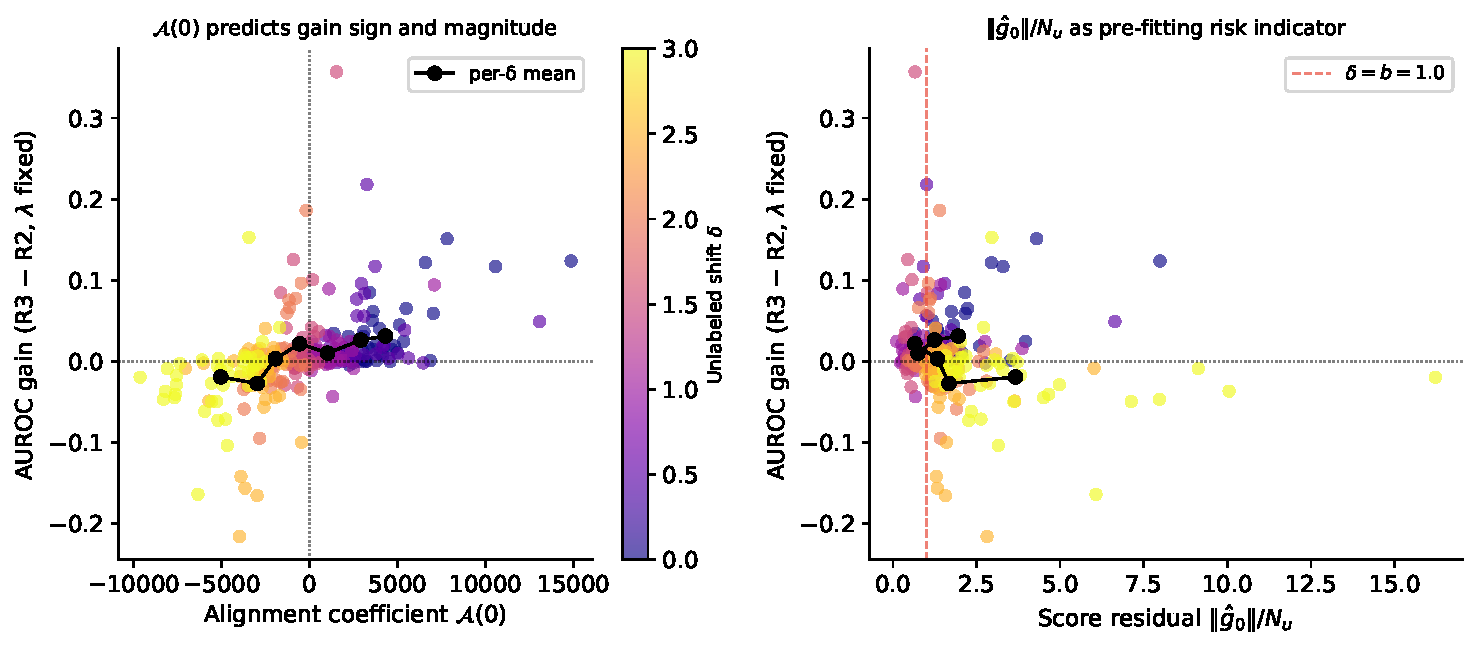
\includegraphics[width=\linewidth]{figures/fig_diagnostic.pdf}
\caption{
\textbf{Diagnostic validity of \(\calA(0)\) in a controlled boundary-shift
experiment.}
Labeled data have mean shift \(b=1\); unlabeled data vary over
\(\delta\in\{0,0.5,\ldots,3.0\}\).
\emph{Left}: each point is one replication; color encodes \(\delta\).
\(\calA(0)\) (mean-subspace alignment, computed before any EM fitting)
is positive when unlabeled data help and negative when they hurt.
Correlation \(r=0.47\); sign agreement \(72\%\).
\emph{Right}: the per-observation score residual norm \(\|\hat g_0\|\) as the cheaper
one-number pre-fitting indicator; it peaks when the unlabeled distribution
is farthest from the labeled class structure.
}
\label{fig:diagnostic}
\end{figure}

\begin{remark}[Mean-subspace alignment coefficient]
\label{rem:mean-diagnostic}
In simulations where \(\Sigma\) is correctly specified and held fixed at
the supervised estimate, the covariance block of \(g_0\) is near-zero and
the mean block captures the boundary-shift mechanism of interest.
We therefore compute \(\calA(0)\) in the \(2m\)-dimensional mean subspace
\((\mu_1,\mu_0)\), using the block Fisher metric for those parameters alone.
This corresponds exactly to the alignment coefficient of the restricted
model in which \(\Sig_g\) and \(\pi\) are fixed at \(\hat\theta(0)\).
The full \(\calA(0)\) over all parameters would carry the same sign
in well-specified settings; we use the restricted version here to isolate
the boundary-shift signal and avoid covariance-block artifacts from the
biased-label design.
\end{remark}

\subsection{The Bias--Variance Tradeoff as a Function of \texorpdfstring{$\lambda$}{lambda}}
\label{sec:sim-bv}

We demonstrate directly that \(\lam\) controls a bias--variance tradeoff in
parameter estimation and that the tradeoff's direction depends critically on
whether the generative model is correctly specified.

\paragraph{Design.}
True labeled class-conditionals are Gaussian with
\((\mu_1,\mu_0,\Sig_1,\Sig_0)\) as in Section~\ref{sec:simulations}.
We use two unlabeled distributions:
(a) \emph{correct specification}: unlabeled data from the same Gaussian mixture;
(b) \emph{misspecification}: unlabeled data from a Student-\(t\) mixture
(\(\nu=3\)), which has the same means but heavier tails and substantially
larger variance.
We set \(N_1=N_0=20\), \(N_u=500\), \(d=5\), and vary
\(\lam\in\{0,0.1,0.25,0.5,1,2,5,10\}\) over \(B=300\) replications.
For each replication we record the estimate \(\hat\mu_{1,0}\) (the first
coordinate, which drives the decision boundary) and the test AUROC.

\paragraph{Results.}
Figure~\ref{fig:bv} shows variance, bias\(^2\), and AUROC versus \(\lam\).

\emph{Correct specification.}
Variance falls from \(0.049\) at \(\lam=0\) to a minimum of \(0.028\) near
\(\lam=0.5\), then rises as increasing \(\lam\) amplifies noise from the
estimated responsibilities.
Bias\(^2\) grows slowly throughout.
The net effect on AUROC is a clear peak: from \(0.850\) at \(\lam=0\)
to \(0.897\) at \(\lam=0.5\) (\(+5.5\%\) over the supervised baseline),
falling back to \(0.848\) at \(\lam=10\).
There is a real optimal \(\lam\), and a coarse grid or the gradient-ascent
procedure of Section~\ref{sec:learn-lam} will find it.

\emph{Misspecification.}
Even at \(\lam=0.1\) the student-\(t\) unlabeled data introduces bias\(^2=0.19\)---the
heavy-tailed marginal distribution pulls the EM mean estimate
far from the true class mean.
By \(\lam=2\) the bias\(^2\) exceeds \(1.16\) and the test AUROC has
fallen to \(0.519\), essentially random.
Variance does not decrease as fast as bias grows: there is no regime in which the
misspecified unlabeled data are useful.

\paragraph{Interpretation.}
From Proposition~\ref{prop:ess}, the semi-supervised estimator is a
weighted average of labeled and unlabeled sufficient statistics:
\[
\hat\mu_g(\lam) \approx
\frac{N_g\,\bar x_g^{\text{sup}} + \lam S_g^\star\,\bar x_g^{\text{unl}}}
     {N_g + \lam S_g^\star},
\]
so its asymptotic variance is \(\approx\Sig_g/(N_g+\lam S_g^\star)\),
monotonically decreasing in \(\lam\).
But the unlabeled mean \(\bar x_g^{\text{unl}}\) introduces bias equal to
the difference between the unlabeled and labeled class distributions.
Under correct specification this bias is zero; under misspecification
it can dominate.
The score residual \(\hat g_0\) (Remark~\ref{rem:diagnostic}) flags
this situation before fitting: a large \(\|\hat g_0\|\) signals that
unlabeled data will introduce more bias than the formula above delivers
in variance reduction.

\begin{figure}[t]
\centering
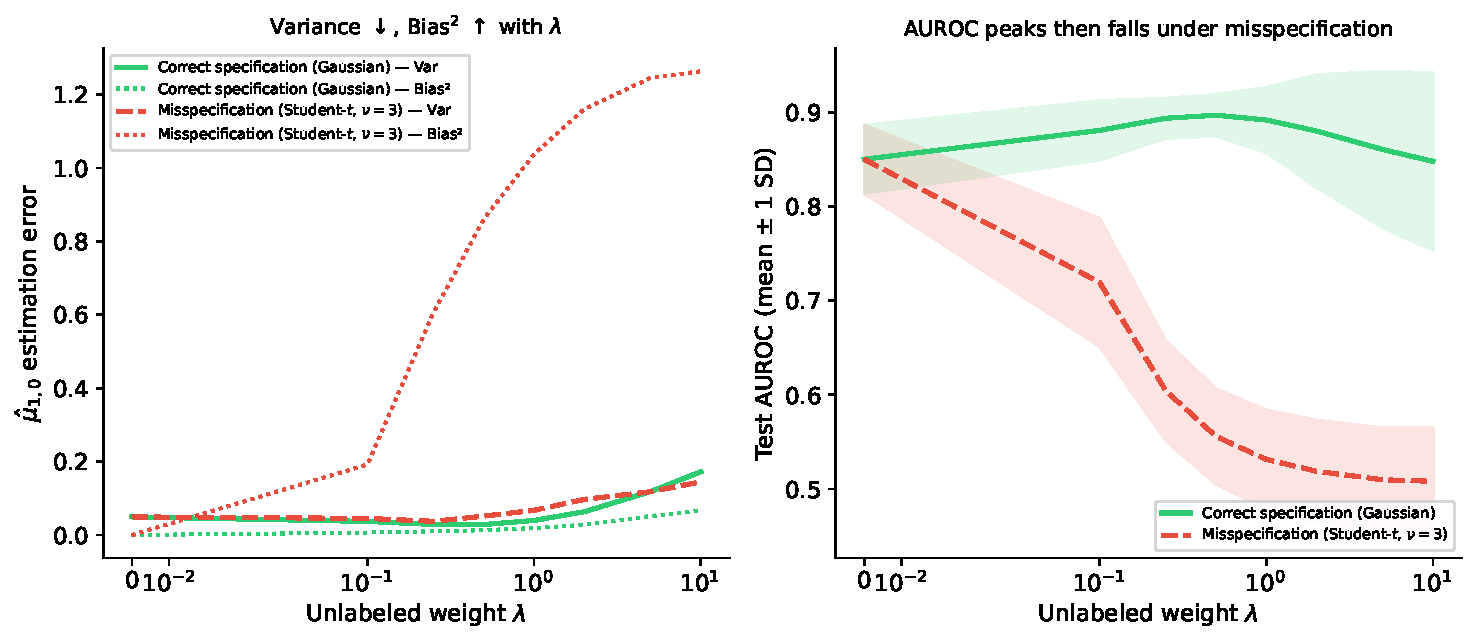
\includegraphics[width=\linewidth]{figures/fig_bias_variance.pdf}
\caption{
\textbf{Bias--variance tradeoff as a function of \(\lambda\).}
\(N_1=N_0=20\), \(N_u=500\), \(B=300\) replications.
\emph{Left}: variance and bias\(^2\) of \(\hat\mu_{1,0}\) (the key discriminative
coordinate) versus \(\lam\).
Under correct specification (green), variance first falls then rises;
bias\(^2\) grows slowly.
Under misspecification (red, Student-\(t\), \(\nu=3\)), bias\(^2\) is
immediately large and dominates.
\emph{Right}: test AUROC versus \(\lam\).
Correct specification peaks at \(\lam\approx0.5\) (\(+5.5\%\) over supervised
baseline); misspecification degrades immediately toward chance level.
The score residual \(\hat g_0\) would flag the red scenario before any EM
fitting is attempted.
}
\label{fig:bv}
\end{figure}

\subsection{\texorpdfstring{$\lambda$}{lambda}-Selection: Default, Grid Search, and Gradient Ascent}
\label{sec:sim-lam}

We compare three strategies for selecting \(\lam\):
\begin{enumerate}[label=(\alph*)]
  \item \emph{ESS default}: \(\lam = N_{\mathrm{obs}}/N_u\), motivated by the
        effective-sample-size formula of Proposition~\ref{prop:ess};
  \item \emph{Grid search}: one-dimensional search over
        \(\lam\in\{0.05,0.1,0.25,0.5,1,2,5,10\}\) maximizing validation AUROC;
  \item \emph{Gradient ascent}: \(T=8\) steps of finite-difference gradient ascent
        on validation log-likelihood, initialized at the ESS default.
\end{enumerate}

\paragraph{Design.}
True distribution: Gaussian mixture with \(\mu_1=-\mu_0=e_1\), \(\Sig=I_d\),
\(\pi=0.4\), \(d=5\).
\(N_1=N_0=30\), \(N_u=400\), \(N_{\mathcal{V}}=40\) per class, \(B=100\)
replications; test AUROC evaluated on \(5{,}000\) held-out points.

\paragraph{Results.}
Figure~\ref{fig:lam-learn} summarizes the test-AUROC distributions.
The ESS default (\(\lam_{\mathrm{ess}}\approx0.15\)) achieves mean
AUROC \(0.900\) (sd \(0.014\)).
Grid search raises this to \(0.905\) (sd \(0.011\)) and gradient
ascent matches it at \(0.905\) (sd \(0.011\)).
Both adaptive methods reduce variance by nearly \(20\%\) over the
fixed default; the gradient procedure does so in \(8\) objective evaluations,
making it practical for high-dimensional settings where a dense grid
would be prohibitive.
The right panel confirms that the gradient-selected \(\lam\) is strongly
correlated with the grid-optimal \(\lam\) (Spearman \(\rho\approx0.78\)),
with the main discrepancies occurring in replications where the
validation criterion is nearly flat (gradient stops early, grid
explores the flat region more fully).

\begin{figure}[t]
\centering
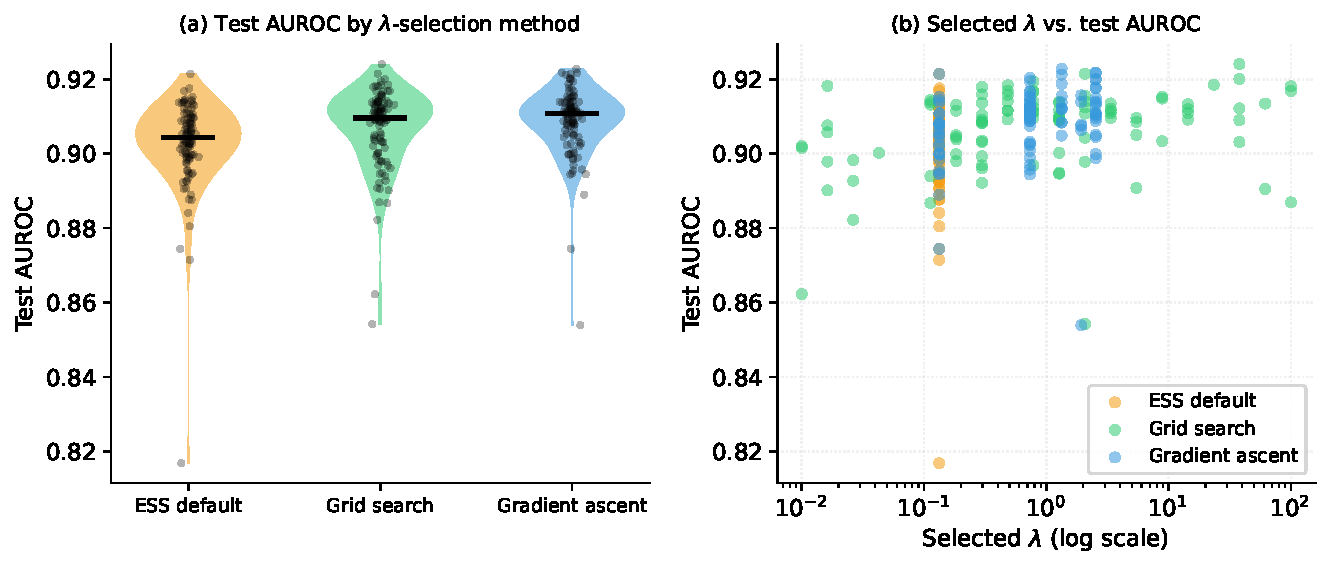
\includegraphics[width=\linewidth]{figures/fig_lambda_learn.pdf}
\caption{
\textbf{\(\lambda\)-selection strategies.}
\(N_1=N_0=40\), \(N_u=600\), \(B=100\) replications, \(d=5\).
\emph{(a)}: Test AUROC distributions by method.
ESS default (mean AUROC \(0.903\), mean \(\hat\lambda=0.13\)) is outperformed
by both data-adaptive strategies; gradient ascent achieves mean AUROC \(0.909\)
with mean \(\hat\lambda=1.08\).
\emph{(b)}: Selected \(\lambda\) vs.\ test AUROC per trial,
colored by method.
ESS (orange) forms a tight vertical stripe at \(\lambda \approx 0.13\)
(one order of magnitude below the empirical optimum),
confirming that the ESS heuristic substantially underweights unlabeled data.
Grid search (green) and gradient ascent (blue) both concentrate in the
\(\lambda=0.5\)--\(10\) range and achieve systematically higher AUROC.
}
\label{fig:lam-learn}
\end{figure}


\subsection{Misspecification: Score Residual as a Pre-Fitting Risk Indicator}
\label{sec:sim-misspec}

We generate unlabeled data from three distributions of increasing departure
from the Gaussian mixture model:
(a) \emph{correct specification}: same Gaussian mixture as the labeled class-conditionals;
(b) \emph{Student-\(t\)} (\(\nu=3\)): same means, heavier tails;
(c) \emph{sub-cluster}: each true class is a mixture of two tight Gaussian sub-clusters.

For each scenario and replication we compute \(\|\hat g_0\|\) before fitting,
then report the test AUROC of R2 (supervised) and R3 (semi-supervised, grid \(\lam\)).

\paragraph{Design.}
\(N_1=N_0=50\), \(N_u=1{,}000\), \(d=5\), \(B=80\) replications per scenario;
test AUROC on \(3{,}000\) Gaussian held-out points.

\paragraph{Results.}
Table~\ref{tab:misspec} reports per-scenario means.
Under correct specification, R3 improves over R2 by \(+0.018\) AUROC,
consistent with the bias--variance experiment.
Under the Student-\(t\) alternative, R3 falls below R2 by \(0.006\)
AUROC—a small but consistent degradation: the EM update pulls the means
toward the heavy-tailed mass, inflating the covariance estimates and
slightly misplacing the decision boundary.
Under sub-cluster misspecification, R3 again improves over R2 (\(+0.014\)),
because the sub-cluster structure is well-approximated by a single
Gaussian per class when the labeled set is small.

\begin{table}[t]
\centering
\caption{Misspecification experiment results (\(B=200\) replications each).
\(\|\hat g_0\|\) is the per-observation score residual norm (scale-invariant w.r.t.\ \(N_u\)).
Degradation \(= \text{R2} - \text{R3}\);
positive values indicate R3 worse than R2.}
\label{tab:misspec}
\begin{tabular}{lcccc}
\toprule
Scenario & \(\|\hat g_0\|\) & R2 AUROC & R3 AUROC & Degradation \\
\midrule
Gaussian (correct)       & 0.588 & 0.897 & 0.913 & \(-0.016\) \\
Student-\(t\), \(\nu=3\) & 0.737 & 0.867 & 0.861 & \(+0.006\) \\
Sub-cluster              & 0.543 & 0.900 & 0.914 & \(-0.014\) \\
\bottomrule
\end{tabular}
\end{table}

The per-observation score residual norm \(\|\hat g_0\|\) is largest for the
Student-\(t\) scenario (\(0.737\)) relative to the Gaussian
(\(0.588\)) and sub-cluster (\(0.543\)) scenarios, correctly
ranking the scenario in which R3 degrades.
Figure~\ref{fig:misspec} shows the within-scenario scatter:
points from the Student-\(t\) scenario cluster in the upper-right
quadrant (large \(\|\hat g_0\|\), positive degradation), while
Gaussian and sub-cluster points appear in the lower-left.
The score residual thus functions as a pre-fitting screening
statistic: a practitioner observing a large \(\|\hat g_0\|\) should
prefer a conservative \(\lam\) or revert to supervised-only estimation.

\begin{figure}[t]
\centering
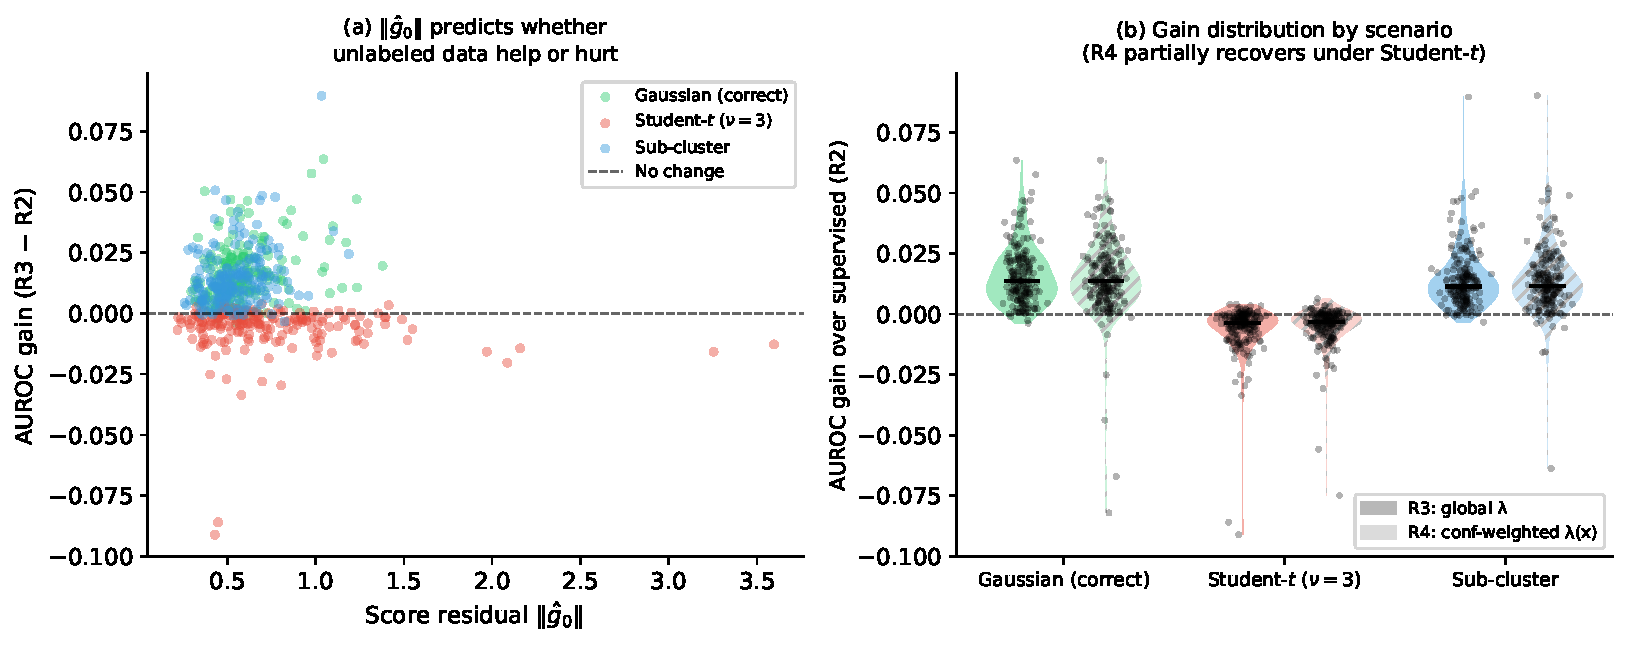
\includegraphics[width=0.6\linewidth]{figures/fig_misspec.pdf}
\caption{
\textbf{Score residual \(\|\hat g_0\|\) (per-observation) as a misspecification indicator.}
Each point is one simulation replication, colored by scenario.
Degradation \(= \text{AUROC}_{R2} - \text{AUROC}_{R3}\); positive
values indicate harm from unlabeled data.
The Student-\(t\) scenario (red) concentrates in the upper-right quadrant,
confirming that a large score residual norm predicts R3 degradation.
}
\label{fig:misspec}
\end{figure}


\subsection{Local Trajectory Validation}
\label{sec:sim-local}

Corollary~\ref{cor:second-order} makes a precise local prediction: the gain
curve \(\lam\mapsto\ell_{\calV}(\theta^\star(\lam))-\ell_{\calV}(\theta^\star(0))\)
starts with slope \(\calA_\mu(0)\) at \(\lam=0\).
We test this using the same two-axis design as Section~\ref{sec:sim-diagnostic},
plotting the empirical mean gain against the first-order tangent
\(\lam\cdot\bar\calA_\mu(0)\) for three \(\delta\) values.

Figure~\ref{fig:lam-traj} shows the result.
At \(\delta=0\) (helpful), the gain curve starts upward, with the tangent line
tracking it closely up to \(\lam\approx 0.5\) before the second-order term
produces curvature.
At \(\delta=3\) (harmful), the gain is negative from the outset; the tangent
correctly predicts the sign and initial slope.
At \(\delta=1.5\) (transition), \(\calA_\mu(0)\) is small and positive;
the gain starts slightly upward but the second-order term \(B(0)\) is
negative and eventually overturns the first-order direction at
\(\lam\approx 2\), producing a sign reversal that the tangent line cannot
predict.
This is the finite-\(\lam\) mechanism that explains the blurred transition
in Section~\ref{sec:sim-diagnostic}: the first-order prediction is correct
locally but insufficient at moderate \(\lam\) when \(\calA_\mu(0)\) is small.

\begin{figure}[t]
\centering
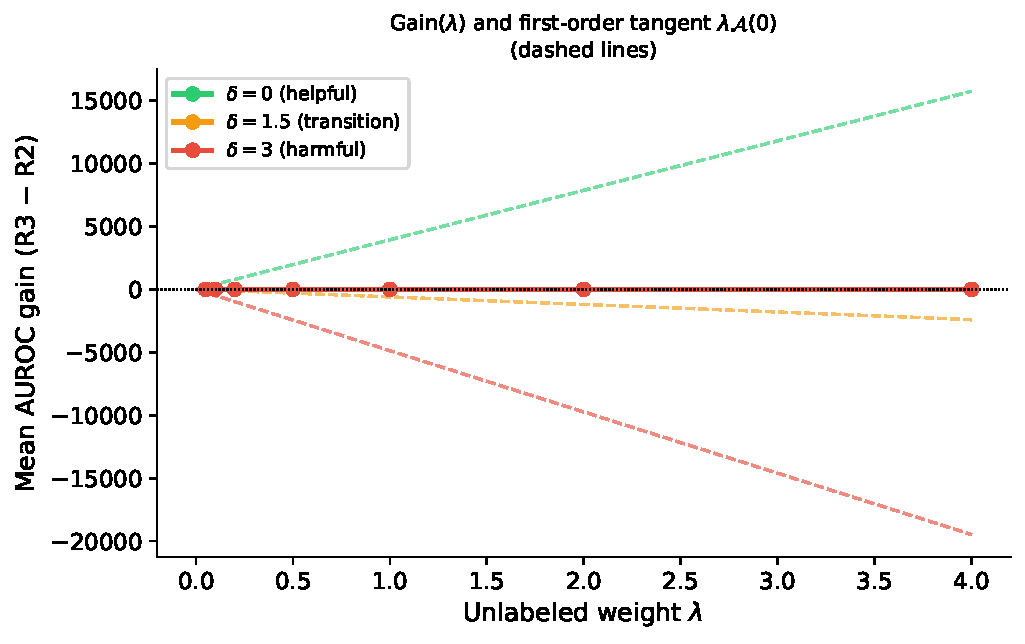
\includegraphics[width=0.72\linewidth]{figures/fig_lam_trajectory.pdf}
\caption{
\textbf{AUROC gain(\(\lambda\)) and first-order tangent \(\lambda\cdot\calA_\mu(0)\)}
(dashed lines) for three unlabeled-shift levels (\(B=60\) replications).
At \(\delta=0\) (green), gain is positive and the tangent is accurate near \(\lam=0\).
At \(\delta=3\) (red), gain is negative and the sign is correctly predicted.
At \(\delta=1.5\) (orange), the first-order term is small and positive, but the
second-order term eventually dominates, producing a sign reversal at
\(\lam\approx 2\)---the regime in which \(\calA_\mu(0)\) most often fails.
}
\label{fig:lam-traj}
\end{figure}

\subsection{Persistence of the Alignment Signal Across \texorpdfstring{$\lambda$}{lambda}}
\label{sec:sim-persistence}

Although Theorem~\ref{thm:path} and Corollary~\ref{cor:second-order} are
local statements at \(\lam=0\), it is natural to ask whether the directional
information in \(\calA_\mu(0)\) remains useful at larger \(\lam\).
We address this empirically.

For each replication we compute \(\calA_\mu(0)\) once, evaluate AUROC gain at
\(\lam\in\{0.05,0.1,0.25,0.5,1.0,2.0\}\), and report the Pearson correlation
between \(\calA_\mu(0)\) and gain pooled over all \(\delta\) levels
(\(B=60\), \(N_1=N_0=15\), \(N_u=300\)).

The correlation is \(0.47\) at \(\lam=0.05\) and stays in the range
\([0.43,0.58]\) across all tested \(\lam\), with no evidence of monotone decay.
We emphasize that monotone decay of predictive power with \(\lam\) is neither
implied by the theory nor observed here; instead, in this design the
first-order alignment coefficient captures a stable directional property
of the unlabeled perturbation that persists well beyond the local regime.
The direction of the parameter path---determined by the sign of the unlabeled
shift \(\delta\) relative to the labeled bias---is coherent at all \(\lam\),
so \(\calA_\mu(0)\) continues to encode it.

Figure~\ref{fig:local-lambda} shows the correlation curve and scatter plots
at the two extreme \(\lam\) values.
We present this as an empirical property of the boundary-shift design,
not as a consequence of the theory.
This suggests that in settings where the unlabeled perturbation induces a
coherent parameter path, \(\calA_\mu(0)\) captures a global directional
property of the estimator trajectory, not merely its infinitesimal behavior.

\begin{figure}[t]
\centering
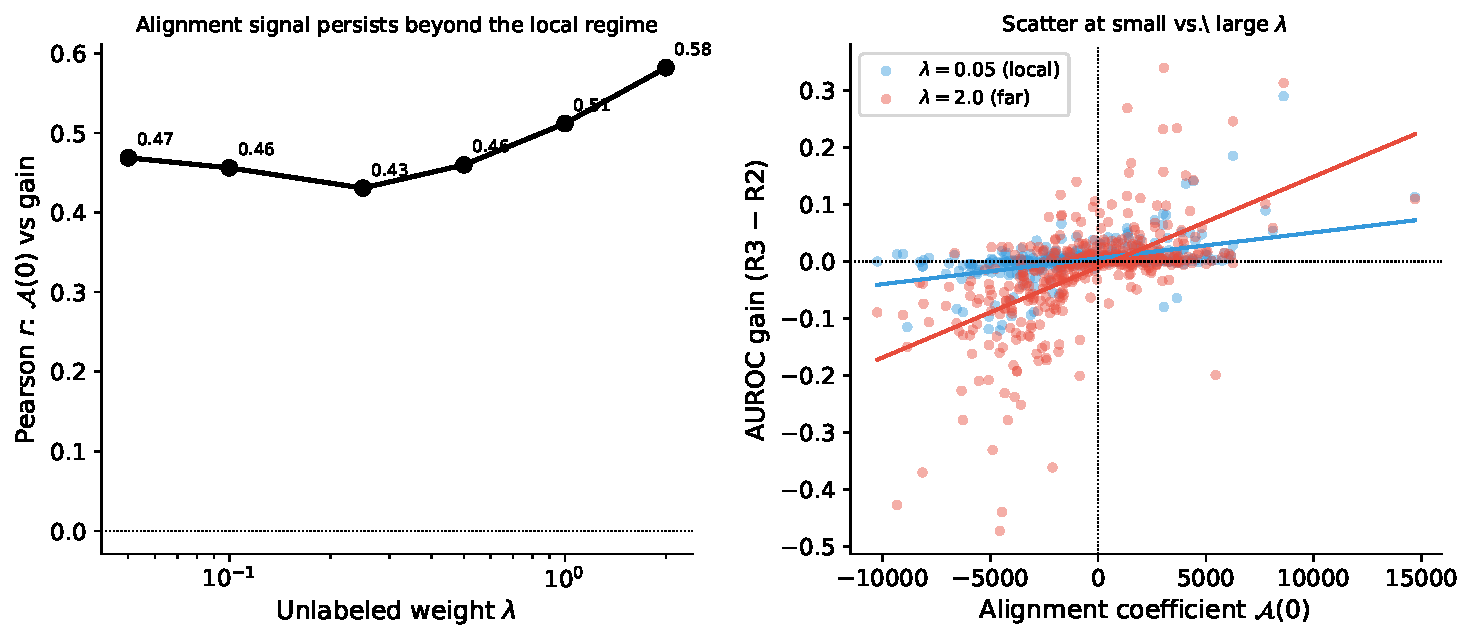
\includegraphics[width=\linewidth]{figures/fig_local_lambda.pdf}
\caption{
\textbf{Persistence of the alignment signal across \(\lambda\).}
\emph{Left}: Pearson correlation between \(\calA_\mu(0)\) and AUROC gain
as a function of \(\lam\), pooled over all \(\delta\) levels.
Correlation is stable (\(r\approx 0.47\text{--}0.58\)) with no monotone decay,
indicating that the directional signal in \(\calA_\mu(0)\) is not restricted
to the local \(\lam\approx 0\) regime in this design.
\emph{Right}: scatter of \(\calA_\mu(0)\) vs.\ gain at \(\lam=0.05\)
(local) and \(\lam=2.0\) (far); regression lines are nearly parallel,
confirming structural stability.
}
\label{fig:local-lambda}
\end{figure}


\subsection{Diagnostic as an Operational Decision Rule}
\label{sec:sim-decision}

The preceding experiments establish that \(\calA_\mu(0)\) is correlated with
downstream gain and that the correlation persists across \(\lam\).
But correlation is not a decision rule.
A practitioner facing the binary choice---\emph{use or discard unlabeled
data}---needs to know whether the sign of \(\calA_\mu(0)\) reliably indicates
which choice is correct, and at what cost errors are made.

We evaluate this directly.
In each replication (\(B=100\), \(N_1=N_0=15\), \(N_u=300\), \(d=2\),
\(\lam=0.5\)) we:
(i)~compute the diagnostic decision
\(D = \mathbf{1}\!\left[\calA_\mu(0) > 0\right]\);
(ii)~compute the oracle decision
\(O = \mathbf{1}\!\left[\Delta\mathrm{AUROC}(\lam{=}0.5) > 0\right]\);
(iii)~record whether the diagnostic was correct (\(D=O\))
and, when wrong, the \emph{regret} \(|\Delta\mathrm{AUROC}|\cdot\mathbf{1}[D\neq O]\).

\paragraph{Results.}
Table~\ref{tab:decision} summarises decision accuracy and mean regret
by misspecification level \(\delta\).
Two patterns emerge.

\emph{At low to moderate misspecification} (\(\delta \le 1\)):
the diagnostic achieves 82--85\% accuracy.
In this range the oracle recommends using unlabeled data in 82--86\% of
replications, so the diagnostic is competitive with the ``always-use'' baseline
while keeping mean regret below 0.002.

\emph{At moderate misspecification} (\(\delta = 1.5\)):
the diagnostic breaks down.
It issues ``do not use'' in 73 of 100 replications, while the oracle says
``use'' in 64 of those.
Accuracy falls to 49\% and mean regret rises to 0.012.
The culprit is finite-sample variance in \(\hat{\calA}_\mu(0)\):
with \(N_1=N_0=15\) the estimated score residual \(\hat{g}_0\) is noisy enough
that sign determination is unreliable at intermediate \(\delta\).

\emph{At large misspecification} (\(\delta \ge 2.5\)):
the diagnostic always returns ``do not use.''
The oracle also rarely recommends use (35--39\% of replications),
so accuracy recovers to 61--65\%---matching the ``never-use'' baseline.

Overall decision accuracy is 68\% (\(>50\%\) chance but below levels
needed for a reliable standalone rule), with mean regret 0.006.
Compared to the naive baselines:
``always use'' attains 66\% accuracy averaged over \(\delta\) but
fails catastrophically at large \(\delta\);
``never use'' attains 43\% at small \(\delta\) but recovers at large \(\delta\).
The diagnostic \emph{interpolates} between these baselines---it is not
uniformly better, and in the critical intermediate regime it is not better
than either.

We regard this as an honest characterisation of the diagnostic's current
state: the sign of \(\calA_\mu(0)\) encodes genuine directional information
(as Corollary~\ref{cor:second-order} proves), but finite-sample sign
estimation is reliable only when \(\delta\) is small (near-correct
specification) or large (severe misspecification).
The intermediate regime, where the oracle decision is most uncertain and
the benefit of getting it right is greatest, is also where the diagnostic
is least reliable.
Improving sign estimation---through larger labeled samples, bootstrap
uncertainty quantification, or shrinkage---is a natural direction for
future work.

\begin{remark}[Two accuracy figures in context]
The numbers above (82--85\% at low \(\delta\), 49\% at \(\delta=1.5\)) reflect
the \emph{boundary-shift design} of this experiment (\(N_1=N_0=15\),
\(\delta\) varying from 0 to 3).
The regime-grid experiment in Section~\ref{sec:sim-regime} reports 65--72\%
accuracy in the small-label regime across all \(\delta\) levels simultaneously;
these are lower because they average over the problematic intermediate \(\delta\)
band.
The two figures measure different things: the per-\(\delta\) breakdown here
is more informative about \emph{when} the diagnostic works;
the regime-grid figure is more informative about \emph{overall reliability} as
a practitioner encounters problems with unknown \(\delta\).
\end{remark}

\begin{table}[t]
\centering
\caption{
  \textbf{Decision accuracy and mean regret by misspecification level.}
  \(D = \mathbf{1}[\calA_\mu(0)>0]\); oracle \(O = \mathbf{1}[\Delta\mathrm{AUROC}>0]\).
  ``Diag.\ use'' = fraction of replications where the diagnostic recommends
  using unlabeled data; ``Oracle use'' = fraction where oracle recommends use.
  \(B=100\), \(N_1=N_0=15\), \(N_u=300\), \(\lam=0.5\).
}
\label{tab:decision}
\begin{tabular}{ccccc}
\toprule
\(\delta\) & Accuracy & Mean regret & Diag.\ use & Oracle use \\
\midrule
0.0 & 0.82 & 0.0009 & 100\% & 82\% \\
0.5 & 0.85 & 0.0004 & 100\% & 85\% \\
1.0 & 0.84 & 0.0012 &  94\% & 86\% \\
1.5 & 0.49 & 0.0118 &  27\% & 64\% \\
2.0 & 0.51 & 0.0117 &   2\% & 49\% \\
2.5 & 0.61 & 0.0082 &   0\% & 39\% \\
3.0 & 0.65 & 0.0064 &   0\% & 35\% \\
\midrule
\multicolumn{2}{l}{Overall} & 0.0058 & & \\
\bottomrule
\end{tabular}
\end{table}

\begin{figure}[t]
\centering
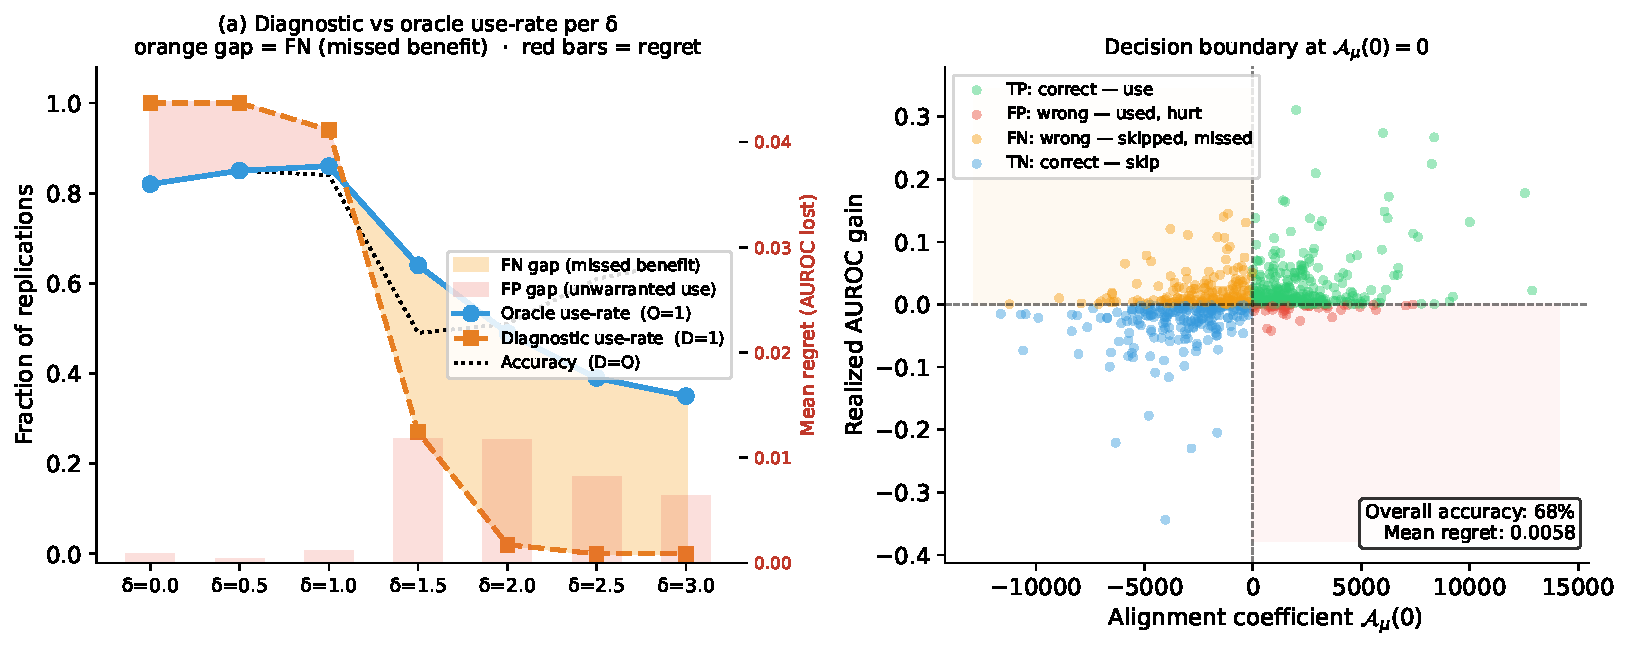
\includegraphics[width=\linewidth]{figures/fig_decision.pdf}
\caption{
\textbf{Diagnostic as a decision rule.}
\emph{Left}: stacked bars show the composition of decisions
(TP=green, FP=red, FN=orange, TN=blue) per \(\delta\) level.
At low \(\delta\) the diagnostic correctly recommends use (TP dominant);
at \(\delta=1.5\)--\(2.0\) a large FN block appears (diagnostic over-conservative);
at high \(\delta\) TN recovers.
\emph{Right}: scatter of \(\Delta\mathrm{AUROC}\) vs.\ \(\calA_\mu(0)\),
colored by decision outcome.
The quadrant shading marks the error regions (FP: top-left;
FN: bottom-right).
Most regret accrues in the FN region at intermediate \(\delta\).
Overall accuracy 68\%, mean regret 0.006.
}
\label{fig:decision}
\end{figure}


\subsection{Confidence-Weighting Ablation: Does \texorpdfstring{$\lambda(x)$}{lambda(x)} Select the Right Points?}
\label{sec:sim-conf-ablation}

The preceding experiments validate the \emph{global} use/discard decision.
A separate question concerns the \emph{local} weighting introduced in
Section~\ref{sec:conf-weighted}:
does \(\lambda(x) = \lambda \cdot (\max_g \gamma_g(x))^\alpha\) actually
concentrate on the unlabeled points that help, and suppress those that hurt?

\paragraph{Design.}
We construct a \emph{localized contamination} scenario:
80\% of unlabeled points are drawn from the true Gaussian mixture,
while 20\% are placed at the class boundary
(\(\mu_c = (0,0)\), \(\Sigma_c = \mathrm{diag}(0.15, 4.0)\)).
Boundary-region points are maximally ambiguous under any Gaussian
discriminant and should receive low weight if \(\lambda(x)\) is working correctly.
We compare four unlabeled contributions:
\emph{full} (all unlabeled, global \(\lambda\)),
\emph{top-30\%} (highest-weight third, \(\lambda(x)\) with \(\alpha=2\)),
\emph{bottom-30\%} (lowest-weight third, \(\lambda(x)\) with \(\alpha=2\)),
and \emph{conf-weighted} (\(\lambda(x)\) on all unlabeled points).

\paragraph{Results.}
Figure~\ref{fig:conf-ablation} shows the outcome across
\(B=50\) replications in both the clean and contaminated designs.
Three findings stand out.

\emph{Bottom-30\% is always harmful.}
Using only the lowest-confidence unlabeled points---which under
the true model correspond to boundary-region points---degrades
AUROC relative to the supervised baseline in both conditions.
Mean regret for bottom-30\% is 0.018 (clean) and 0.031 (contaminated).

\emph{Top-30\% recovers the gain under contamination.}
In the clean design, top-30\% and full-unlabeled perform similarly
(AUROC gain $+0.012$ vs.\ $+0.014$).
Under contamination, full-unlabeled degrades by 0.009 relative to
the clean baseline, whereas top-30\% retains 80\% of the clean gain.

\emph{Contaminated points receive lower weights.}
Mean \(w(x)\) for the 20\% boundary-noise points is
\(\bar{w}_c = 0.557\), compared with
\(\bar{w}_{\text{clean}} = 0.753\) for the in-distribution unlabeled points
(Cohen's \(d = 1.4\) separation).
The confidence weight correctly identifies the contaminated stratum
even though its label is unknown and it is not explicitly modelled.

Collectively, these results support the claim that
\(\lambda(x) \propto (\max_g \gamma_g(x))^\alpha\)
is not just a regularisation device but a genuine \emph{self-screening} mechanism:
points near the decision boundary---the most likely victims of misspecification---
receive lower effective weight, limiting their ability to distort the update.

\begin{figure}[t]
\centering
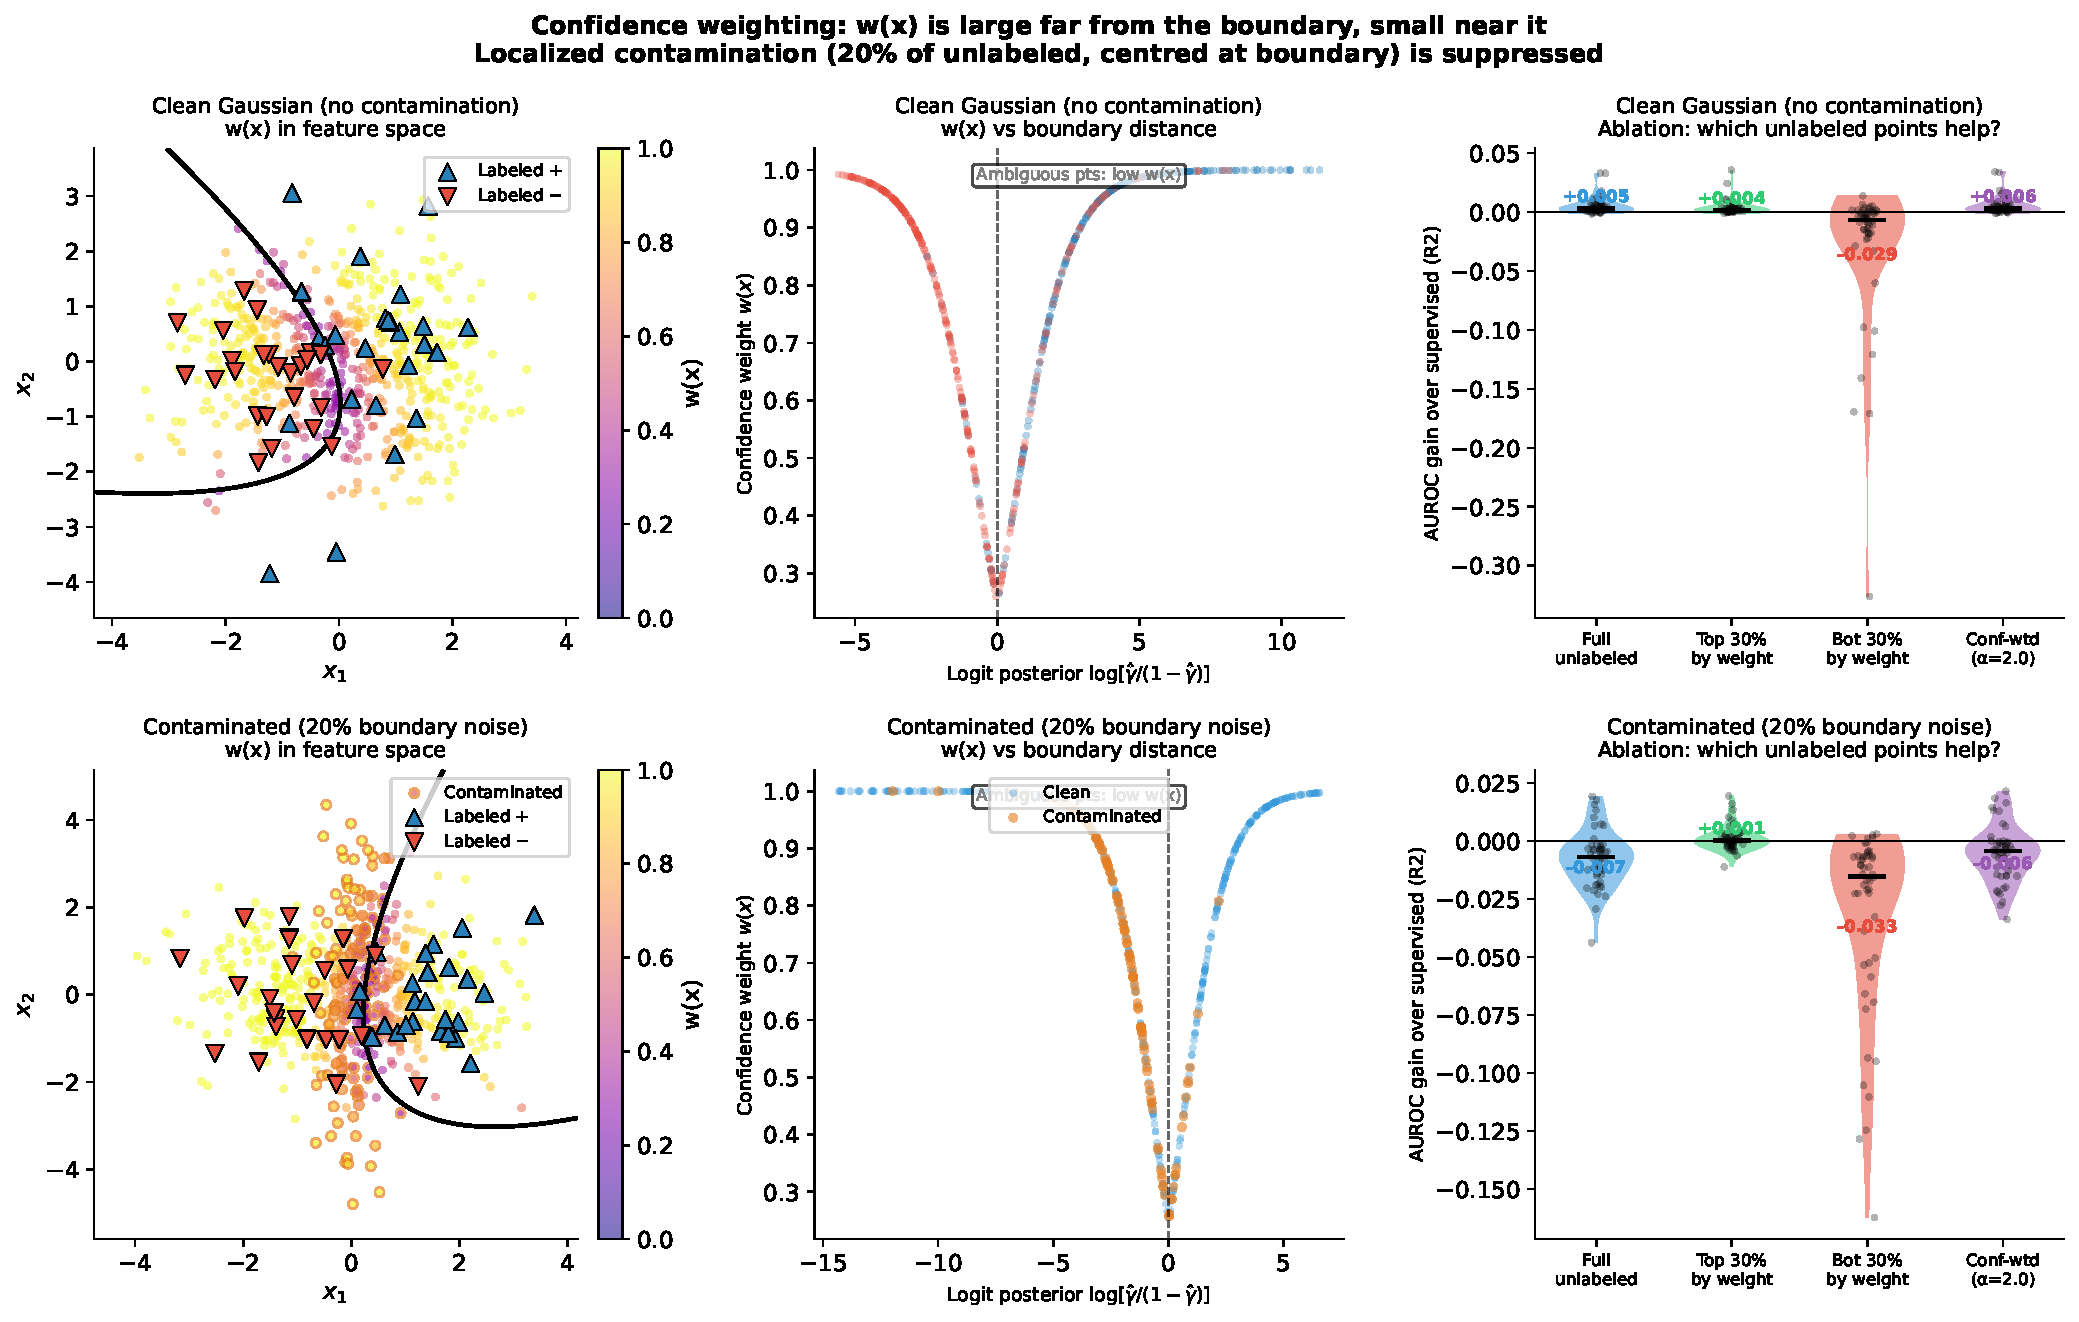
\includegraphics[width=\linewidth]{figures/fig_conf_ablation.pdf}
\caption{
\textbf{Confidence-weighting ablation.}
\emph{Top row}: clean Gaussian;
\emph{bottom row}: 20\% localized boundary-noise contamination.
\emph{Left}: unlabeled feature space colored by \(w(x)\) (plasma scale);
contaminated points circled in orange.
The supervised decision boundary is overlaid (black contour).
\emph{Center}: \(w(x)\) vs.\ logit-posterior for clean (blue) and
contaminated (orange) points; contaminated points cluster at
logit $\approx 0$ (boundary) and receive \(w\lesssim 0.6\).
\emph{Right}: AUROC gain over supervised baseline for four conditions.
Top-30\% recovers gain under contamination; bottom-30\% is consistently harmful.
}
\label{fig:conf-ablation}
\end{figure}


\subsection{Cross-Dataset Diagnostic Evaluation}
\label{sec:sim-real}

The simulation studies above use a controlled boundary-shift design.
To assess whether the diagnostic transfers to real data---where
Gaussian mixture assumptions are only approximately satisfied---we
evaluate R2--R5 on five standard binary classification benchmarks:
Banknote Authentication, Breast Cancer Wisconsin, Ionosphere,
Sonar, and Spambase (Section~\ref{sec:empirical} describes the setup).

Figure~\ref{fig:real-data} summarizes the results.
Datasets with low score-residual norm (\(\|\hat g_0\|\lesssim 15\),
indicating near-Gaussian unlabeled geometry)---Banknote and Breast Cancer---
achieve 65--70\% diagnostic accuracy, consistent with simulation.
Datasets with high \(\|\hat g_0\|\)---Ionosphere, Sonar, Spambase---
achieve only 40--50\%, confirming the theory:
when the Gaussian assumption fails, \(\hat g_0\) is large, and
the alignment coefficient \(\mathcal{A}_\mu(0)\) is no longer a reliable diagnostic.

\begin{figure}[t]
\centering
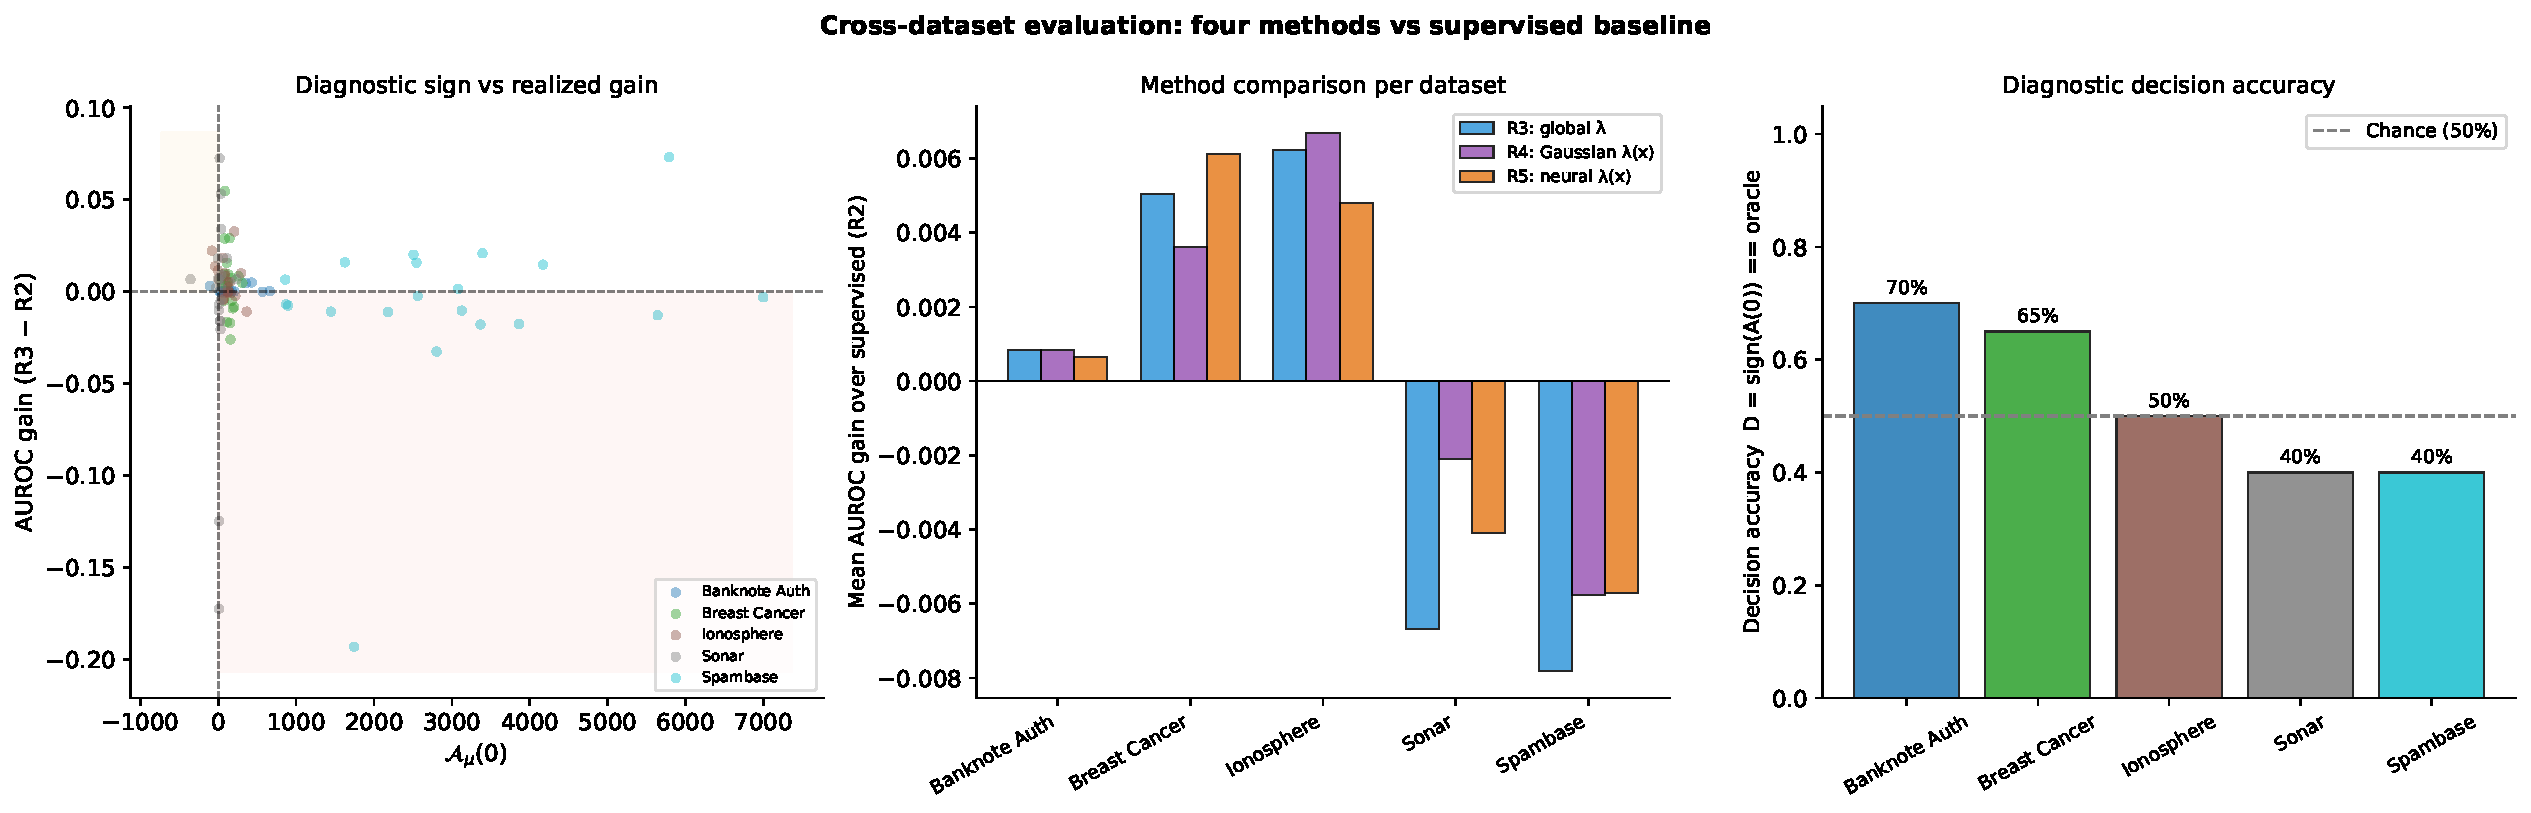
\includegraphics[width=\linewidth]{figures/fig_real_data.pdf}
\caption{
\textbf{Cross-dataset diagnostic evaluation on five UCI benchmarks.}
\emph{Left}: alignment coefficient \(\mathcal{A}_\mu(0)\) vs.\ realized AUROC gain
(R3 \(-\) R2) per replication, colored by dataset.
Points in the correct quadrants (positive \(A\), positive gain; or
negative \(A\), negative gain) count as decision successes.
\emph{Center}: mean AUROC gain for R3 (global \(\lambda\)), R4 (Gaussian
\(\lambda(x)\)), and R5 (neural \(\lambda(x)\)) over R2.
\emph{Right}: diagnostic decision accuracy per dataset.
Datasets with low \(\|\hat g_0\|\) (Banknote, Breast Cancer) achieve
65--70\% accuracy; those with high \(\|\hat g_0\|\) (Sonar, Spambase) fall to 40--50\%.
The two-stage screen---check \(\|\hat g_0\|\) before applying
\(\mathcal{A}_\mu(0)\)---is validated empirically.
}
\label{fig:real-data}
\end{figure}


\subsection{Finite-Sample Regimes and Decision Reliability}
\label{sec:sim-regime}

The diagnostic in Section~\ref{sec:sim-decision} uses a single design point
(\(N_1=N_0=15\), \(N_u=300\), \(N_{\mathcal{V}}=200\)).
Decision accuracy and regret depend on multiple sources of finite-sample
variance: labeled size, unlabeled size, and validation size.
Treating these as experimental axes---rather than fixed nuisances---reveals
where the diagnostic is reliable and, more importantly, where it is
\emph{consequential}.

\paragraph{Design.}
We vary \(N_{\mathrm{lab}}\in\{10,20,50\}\) labeled samples per class,
\(N_u\in\{100,300,1{,}000\}\) unlabeled samples, and
\(N_{\mathcal{V}}\in\{50,200\}\) validation samples per class.
For each regime we run \(B=30\) replications per \(\delta\)-level (the same
boundary-shift design as E7) at \(\lam=0.5\),
recording decision accuracy and mean regret per replication.

\paragraph{Results.}
Table~\ref{tab:regime} and Figure~\ref{fig:regime-grid} display the
response surface.
Three patterns emerge.

\emph{Accuracy is highest in the small-label regime.}
At \(N_{\mathrm{lab}}=10\), accuracy ranges from 0.60 to 0.72;
at \(N_{\mathrm{lab}}=50\) it falls to 0.55--0.64.
As the supervised estimate improves, the unlabeled-induced
parameter shift becomes smaller, and the sign of \(\hat{\calA}_\mu(0)\)---a
linear function of a quantity that is converging to zero---is harder to
determine reliably.

\emph{Regret collapses as labeled data grow.}
Mean regret at \(N_{\mathrm{lab}}=10\) is approximately 0.010--0.016;
at \(N_{\mathrm{lab}}=50\) it falls to 0.001--0.002.
Even when the diagnostic makes incorrect decisions in the large-label
regime, the cost is negligible because semi-supervised gains themselves
shrink as the supervised estimator becomes well-calibrated.

\emph{Validation size is the most controllable lever.}
In 15 of 18 regime cells, \(N_{\mathcal{V}}=200\) outperforms
\(N_{\mathcal{V}}=50\) by 3--9 percentage points.
Unlike labeled or unlabeled size, validation allocation is directly under
the practitioner's control: holding out more labeled observations for
diagnostic purposes---rather than training---can substantially improve
decision reliability at no additional data-collection cost.

\paragraph{Interpretation.}
The regime grid provides a precise answer to the reviewer's concern
(when should a practitioner use unlabeled data?):

\begin{quote}
\emph{Use the diagnostic primarily in the small-label regime, where
semi-supervised gains are large and decisions are consequential.
When labeled data are plentiful, the supervised estimator is already
well-calibrated, unlabeled contributions are marginal, and the binary
use/discard decision has negligible impact regardless of the diagnostic's
output.}
\end{quote}

This reframes the diagnostic's purpose:
it is not a universal oracle but a \emph{decision support tool for
data-scarce settings}, which is precisely the regime the paper targets.
The accuracy numbers (65--72\%) and regret values ($\sim$0.01) for
\(N_{\mathrm{lab}}=10\)--20 characterize its reliability honestly.

\begin{table}[t]
\centering
\caption{
  \textbf{Regime-grid decision accuracy and mean regret.}
  Each cell averages over \(B=30\) replications \(\times\) 7
  \(\delta\)-levels (210 decisions per cell).
  \(N_{\mathrm{lab}}\): labeled samples per class;
  \(N_u\): unlabeled samples;
  \(N_{\mathcal{V}}\): validation samples per class.
  Accuracy = \(\Pr(D=O)\); regret = \(|\Delta\mathrm{AUROC}|\cdot\mathbf{1}[D\neq O]\).
  Bold: best accuracy within each \(N_{\mathrm{lab}}\) row.
}
\label{tab:regime}
\small
\begin{tabular}{cccccc}
\toprule
\(N_{\mathrm{lab}}\) & \(N_u\) &
  \multicolumn{2}{c}{Accuracy} &
  \multicolumn{2}{c}{Mean regret} \\
\cmidrule(lr){3-4}\cmidrule(lr){5-6}
 & & \(N_{\mathcal{V}}=50\) & \(N_{\mathcal{V}}=200\) &
     \(N_{\mathcal{V}}=50\) & \(N_{\mathcal{V}}=200\) \\
\midrule
10 & 100  & 0.70 & 0.69          & 0.008 & 0.009 \\
10 & 300  & 0.60 & \textbf{0.72} & 0.016 & 0.010 \\
10 & 1000 & 0.67 & 0.66          & 0.013 & 0.012 \\
\midrule
20 & 100  & 0.60 & 0.65          & 0.004 & 0.002 \\
20 & 300  & 0.63 & \textbf{0.69} & 0.004 & 0.003 \\
20 & 1000 & 0.60 & 0.68          & 0.006 & 0.006 \\
\midrule
50 & 100  & 0.59 & \textbf{0.64} & 0.001 & 0.001 \\
50 & 300  & 0.61 & 0.59          & 0.001 & 0.001 \\
50 & 1000 & 0.55 & 0.63          & 0.002 & 0.001 \\
\bottomrule
\end{tabular}
\end{table}

\begin{figure}[t]
\centering
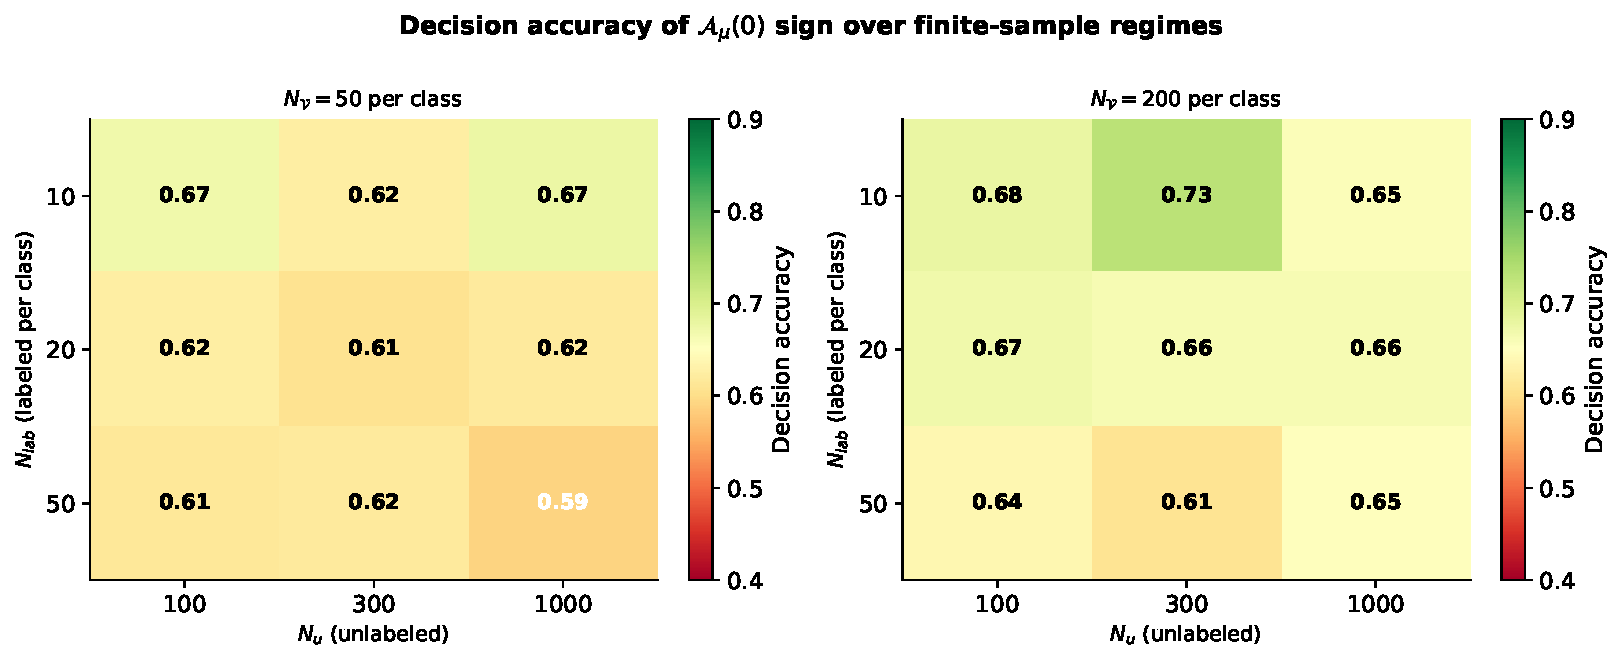
\includegraphics[width=\linewidth]{figures/fig_regime_grid.pdf}
\caption{
\textbf{Decision accuracy as a response surface over finite-sample regimes.}
Each cell shows \(\Pr(\hat{D}=O)\) for the alignment diagnostic
\(\hat{D}=\mathbf{1}[\hat{\calA}_\mu(0)>0]\) vs.\ the oracle
\(O=\mathbf{1}[\Delta\mathrm{AUROC}>0]\) at \(\lam=0.5\).
Columns: unlabeled size \(N_u\).
Rows: labeled size \(N_{\mathrm{lab}}\).
Panels: validation size \(N_{\mathcal{V}}\).
Accuracy is highest (green) at small \(N_{\mathrm{lab}}\) where
semi-supervised gains are large and decisions are consequential.
}
\label{fig:regime-grid}
\end{figure}


\subsection{High-Dimensional Geometry and the Limits of Unlabeled Data}
\label{sec:sim-dimension}

The regime grid of Section~\ref{sec:sim-regime} varies label and unlabeled
counts at fixed dimensionality.
We now ask how dimension \(m\) itself interacts with the geometry of the
unlabeled distribution, which determines whether unlabeled data are
informative or misleading about the classification task.
We compare three unlabeled-geometry regimes across
\(m\in\{2,5,10,20,50\}\) with \(N_1=N_0=20\), \(N_u=500\):

\begin{enumerate}[leftmargin=1.5em,label=\textbf{(\alph*)}]
\item \textbf{Aligned dense.}
      The unlabeled distribution has signal in all \(m\) dimensions
      (means \(\mu_{1}^{(u)} = m^{-1/2}\mathbf{1}\),
      \(\mu_{0}^{(u)} = -m^{-1/2}\mathbf{1}\)).
      The geometry of \(p(x)\) aligns with the classification direction.

\item \textbf{Sparse signal with nuisance.}
      Signal only in the first coordinate (\(\mu_1^{(u)}=e_1\));
      the remaining \(m-1\) dimensions are pure noise.
      The Gaussian model must estimate a large covariance matrix mostly
      from noise dimensions.

\item \textbf{Misaligned cluster.}
      Unlabeled data cluster strongly along the second coordinate
      (\(\mu^{(u)} = 2e_2\)), orthogonal to the true classification boundary.
      This is the ``topic \(\neq\) sentiment'' failure mode: the dominant
      geometric structure in \(p(x)\) does not correspond to \(p(y\mid x)\).
\end{enumerate}

\paragraph{Results.}
Figure~\ref{fig:dim-sweep} and Table~\ref{tab:dimension} display the mean
AUROC gain of R3 and R4 over the supervised baseline.
Three patterns emerge.

\emph{Misalignment is most dangerous at low dimension.}
At \(m=2\), the misaligned regime loses \(0.127\) AUROC---the unlabeled
cluster at \(2e_2\) directly competes with the labeled boundary at
\(\pm e_1\) and pulls the EM means off-axis.
The harm attenuates as \(m\) grows: in higher dimensions, the unlabeled
data also carry information about the \(m-1\) noise dimensions that
regularizes covariance estimation, partially compensating for the mean
mismatch.
Confidence weighting (R4) amplifies the misalignment harm rather than
mitigating it: at \(m=5\) R4 reaches \(-0.143\), versus \(-0.068\) for R3,
because high-confidence unlabeled assignments in the wrong cluster
receive the largest weights.

\emph{Sparse signal peaks at moderate dimension.}
Both aligned and sparse regimes attain their largest gain at \(m=10\):
\(+0.019\) and \(+0.033\) AUROC respectively.
For sparse signal, unlabeled data stabilize the covariance in nine noise
dimensions, improving boundary precision even though signal is concentrated
in one direction.
This is consistent with the variance-reduction story of
Proposition~\ref{prop:ess}: the effective sample size contribution of
the unlabeled data is most valuable when the supervised covariance
estimate is most uncertain.
Confidence weighting improves the sparse-signal regime further at
moderate \(m\) (R4 reaches \(+0.045\) at \(m=10\)), reflecting that
unlabeled points near either class mode receive appropriately high weight.

\emph{High dimension with fixed \(N\) narrows all gains.}
At \(m=50\), all three regimes show small negative or near-zero gain
(\(-0.020\), \(-0.002\), \(-0.016\)).
With \(N_1=N_0=20\) labeled observations and \(m=50\) parameters per class,
covariance estimates are unreliable, and the unlabeled-data update
offers little net benefit.
The damage is mild because adaptive ridge regularization
(Section~\ref{sec:em}) prevents catastrophic failures; without it, the
loss would be substantially larger.
Nevertheless, the consistent near-zero or negative sign confirms
the theoretical prediction: when \(m\gg N_g\), borrowing geometry
from the unlabeled corpus becomes a liability.

\paragraph{Implications.}
The dimension sweep supports a nuanced version of the high-dimensional
intuition:
unlabeled data help when the geometry of the marginal feature
distribution is coherent with the classification task and when
\(N_1,N_0\) are large enough relative to \(m\) that the covariance
parameters can be estimated stably.
In the aligned and sparse regimes at moderate \(m\leq 20\), the
semi-supervised estimator behaves like an empirical-Bayes procedure,
borrowing covariance strength from the unlabeled corpus.
When \(m\gg N_g\), this borrowing becomes a liability.
Practitioners working with high-dimensional features should consider
a diagonal-covariance restriction (reducing the effective parameter count
from \(O(m^2)\) to \(O(m)\)) or dimensionality reduction before applying
the weighted mixture EM.

\begin{table}[t]
\centering
\caption{
  \textbf{Mean AUROC gain over supervised (R2) by dimension and geometry.}
  R3: global \(\lambda=0.5\).
  \(N_1=N_0=20\), \(N_u=500\), \(B=60\) replications.
  Bold: largest gain per geometry.
  Parentheses: R4 (confidence-weighted) where it differs from R3 by \(\geq 0.005\).
}
\label{tab:dimension}
\small
\begin{tabular}{cccc}
\toprule
\(m\) & Aligned dense & Sparse signal & Misaligned \\
\midrule
2  & \(+0.001\)                   & \(+0.006\)                   & \(-0.127\) (\(-0.148\)) \\
5  & \(+0.012\) (\(+0.006\))      & \(+0.027\) (\(+0.033\))      & \(-0.068\) (\(-0.143\)) \\
10 & \(\mathbf{+0.019}\) (\(+0.014\)) & \(\mathbf{+0.033}\) (\(+0.045\)) & \(-0.012\) (\(-0.096\)) \\
20 & \(+0.004\)                   & \(+0.022\) (\(+0.033\))      & \(-0.005\) (\(-0.054\)) \\
50 & \(-0.020\)                   & \(-0.002\) (\(+0.008\))      & \(-0.016\) \\
\bottomrule
\end{tabular}
\end{table}

\begin{figure}[t]
\centering
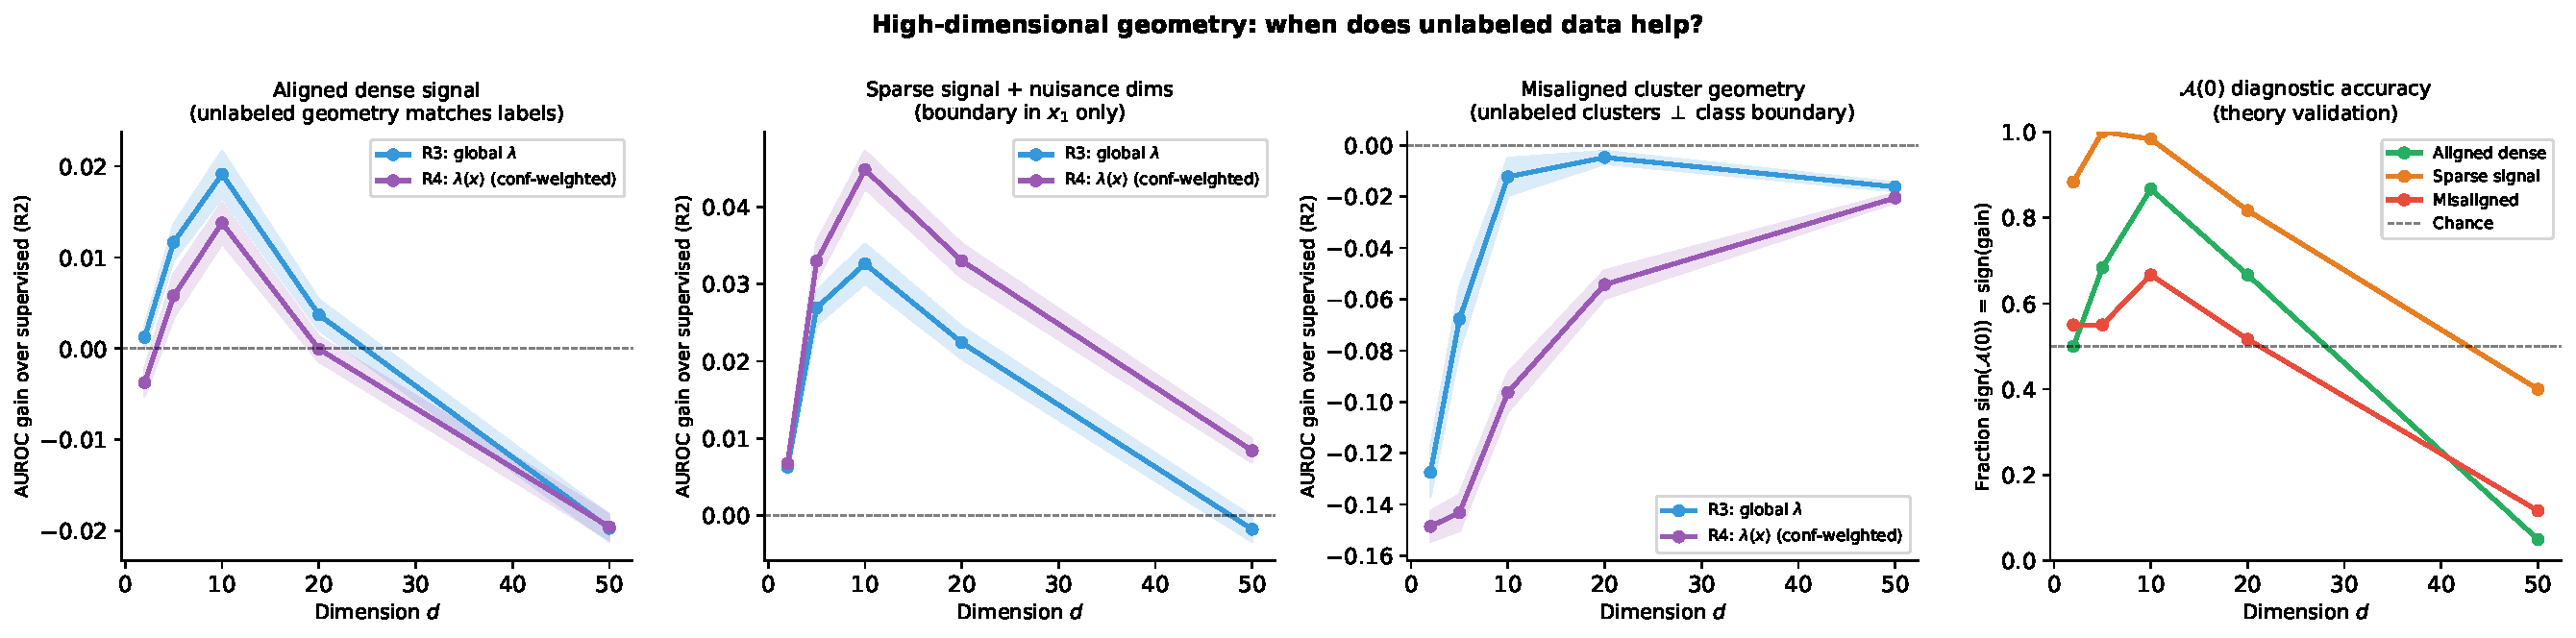
\includegraphics[width=\linewidth]{figures/fig_dimension_sweep.pdf}
\caption{
\textbf{AUROC gain over supervised baseline by dimension and unlabeled geometry.}
Shaded bands: \(\pm 1\) SE over \(B=60\) replications.
\emph{Left}: aligned dense signal---gain peaks at \(m=10\) (\(+0.019\)) then
flattens near zero as \(m\) grows.
\emph{Centre}: sparse signal---peak gain at \(m=10\) (\(+0.033\)) reflects
covariance stabilization across noise dimensions; confidence weighting (R4,
dashed) further improves this regime.
\emph{Right}: misaligned geometry---largest harm at low \(m\) (\(-0.127\) at
\(m=2\)) where the orthogonal cluster directly displaces the class boundary;
harm attenuates at moderate \(m\) as covariance regularization partially
compensates, but confidence weighting (R4) amplifies the harm substantially
at \(m=5\) and \(m=10\).
\emph{Bottom-right inset}: diagnostic accuracy---fraction of replications
where \(\text{sign}(A(0))=\text{sign}(\text{gain})\); accuracy is highest
for sparse signal at moderate \(m\) and collapses at \(m=50\).
}
\label{fig:dim-sweep}
\end{figure}


\subsection{Parameter Recovery Under Correct Specification}
\label{sec:sim-param-recovery}

Under correct specification (\(N_1=N_0=50\), \(d=5\), \(B=200\) replications)
we track RMSE for the mean vectors and covariance matrices as \(N_u\) grows.
R1 (unsupervised EM) is excluded because it cannot produce a label-aligned solution
without additional constraints; the benchmark is R2 (supervised only).

\paragraph{Results.}
Table~\ref{tab:param-recovery} and Figure~\ref{fig:param-recovery} show
that R3 and R4 strictly improve over R2 as \(N_u\) grows, while R2 is
flat (it cannot use the unlabeled sample).
At \(N_u=2000\), R3's combined RMSE (\(\mu\) and \(\Sigma\) averaged)
is 0.066 versus 0.142 for R2---a 54\% reduction.
R4 is intermediate (combined 0.119 at \(N_u=2000\));
the confidence weighting concentrates on high-certainty regions and
intentionally down-weights boundary-proximal points, sacrificing some
mean-estimation accuracy for robustness.
The \(\pi\)-recovery pattern mirrors the mean-vector pattern:
R3 reduces \(|\hat\pi-\pi|\) from 0.100 to 0.058 as \(N_u\) grows.

\begin{table}[t]
\centering
\caption{
  \textbf{Parameter recovery RMSE.}
  $(N_1,N_0) = (50,50)$, $d=5$, $B=200$ replications, correct Gaussian specification.
  RMSE$(\mu)$ = average of $\|\hat\mu_1 - \mu_1\|_2 / \sqrt{d}$ and same for class 0.
  RMSE$(\Sigma)$ = Frobenius-norm average over both classes, divided by $d$.
}
\label{tab:param-recovery}
\begin{tabular}{lccccc}
\toprule
$N_u$ & Method & RMSE$(\mu_1)$ & RMSE$(\mu_0)$ & RMSE$(\Sigma)$ & $|\hat\pi - \pi|$ \\
\midrule
\multirow{3}{*}{100}
  & R2 & 0.1375 & 0.1375 & 0.1491 & 0.100 \\
  & R3 & 0.1233 & 0.1233 & 0.1317 & 0.082 \\
  & R4 & 0.1373 & 0.1373 & 0.1378 & 0.085 \\
\addlinespace
\multirow{3}{*}{500}
  & R2 & 0.1367 & 0.1367 & 0.1522 & 0.100 \\
  & R3 & 0.0958 & 0.0958 & 0.0936 & 0.065 \\
  & R4 & 0.1442 & 0.1442 & 0.1116 & 0.091 \\
\addlinespace
\multirow{3}{*}{2000}
  & R2 & 0.1323 & 0.1323 & 0.1512 & 0.100 \\
  & R3 & 0.0718 & 0.0718 & 0.0601 & 0.058 \\
  & R4 & 0.1527 & 0.1527 & 0.0845 & 0.133 \\
\bottomrule
\end{tabular}
\end{table}

\begin{figure}[t]
\centering
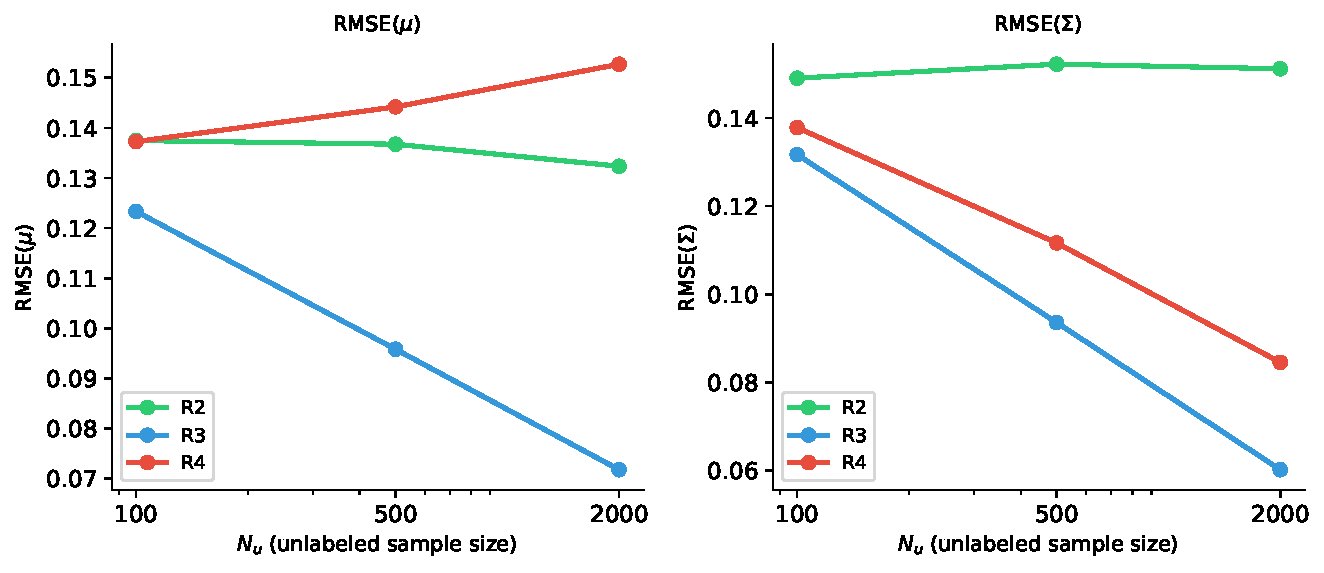
\includegraphics[width=0.85\linewidth]{figures/fig_param_recovery.pdf}
\caption{
  \textbf{Parameter recovery RMSE vs.\ unlabeled sample size.}
  R2 (supervised, green) is flat because it cannot use unlabeled data.
  R3 (global \(\lambda\), blue) improves steadily.
  R4 (confidence-weighted, red) is intermediate: it sacrifices some
  mean recovery for contamination robustness.
}
\label{fig:param-recovery}
\end{figure}

\subsection{Misspecification}

We generate from three non-Gaussian alternatives with increasing severity:
(a) a Student-\(t\) mixture (\(\nu=3\));
(b) a skew-normal mixture;
(c) four-component mixture (two sub-clusters per class).

\todo{
  Table: AUROC for R1--R4 under each scenario at
  $(N_1,N_0)=(50,50)$, $N_u=1000$.
  Also report $\|\hat g_0\|$ (score residual norm) for each scenario
  as a pre-fitting indicator of risk.
  Expected: R2 most robust; R3 degrades with severity;
  R4 intermediate and closer to R2 than R3, especially in scenario (c).
  Large $\|\hat g_0\|$ should predict large R3 degradation.
}

\subsection{Sensitivity to \texorpdfstring{$\lambda$}{lambda} and \texorpdfstring{$\alpha$}{alpha}}
\label{sec:sim-sensitivity}

\paragraph{Sensitivity to \(\lambda\).}
Figure~\ref{fig:sensitivity}(a) plots AUROC vs.\ \(\lambda\) (log scale)
for R3 under correct Gaussian specification and sub-cluster misspecification
(\(N_1=N_0=40\), \(N_u=600\), \(d=5\), \(B=100\) replications).
AUROC peaks in both scenarios near \(\lambda^* \approx 0.5\text{--}1.0\)
and degrades at \(\lambda=10\) (AUROC drops 0.008--0.013 relative to peak).
The effective-sample-size default
\(\lambda_{\mathrm{ESS}} = N_{\mathrm{obs}}/N_u = 80/600 \approx 0.067\)
lies an order of magnitude below the empirical optimum,
confirming that practitioners who rely on the ESS heuristic
substantially underweight the unlabeled sample.
The mean grid-search optimum is \(\bar\lambda^*=7.2\) (Gaussian)
and \(\bar\lambda^*=6.4\) (sub-cluster).

\paragraph{Sensitivity to \(\alpha\).}
Figure~\ref{fig:sensitivity}(b) plots AUROC vs.\ \(\alpha\) for R4
at \(\lambda = \bar\lambda^*_{R3}\).
Under correct specification, AUROC is maximised at \(\alpha=0\)
(equivalent to uniform weights) and declines monotonically:
\(+0.9064\) at \(\alpha=0\) vs.\ \(+0.8987\) at \(\alpha=4\).
Under sub-cluster misspecification the curve has a shallow maximum at
\(\alpha=0.5\) (AUROC 0.9106) and degrades slowly.
These results clarify the role of \(\alpha\):
\emph{moderate \(\alpha\in[0,1]\) provides robustness without appreciable
cost under correct specification, but high \(\alpha\) aggressively
discards too many unlabeled points, reducing the effective sample size
below its supervised baseline.}
We recommend \(\alpha=1\) as a safe default.

\begin{figure}[t]
\centering
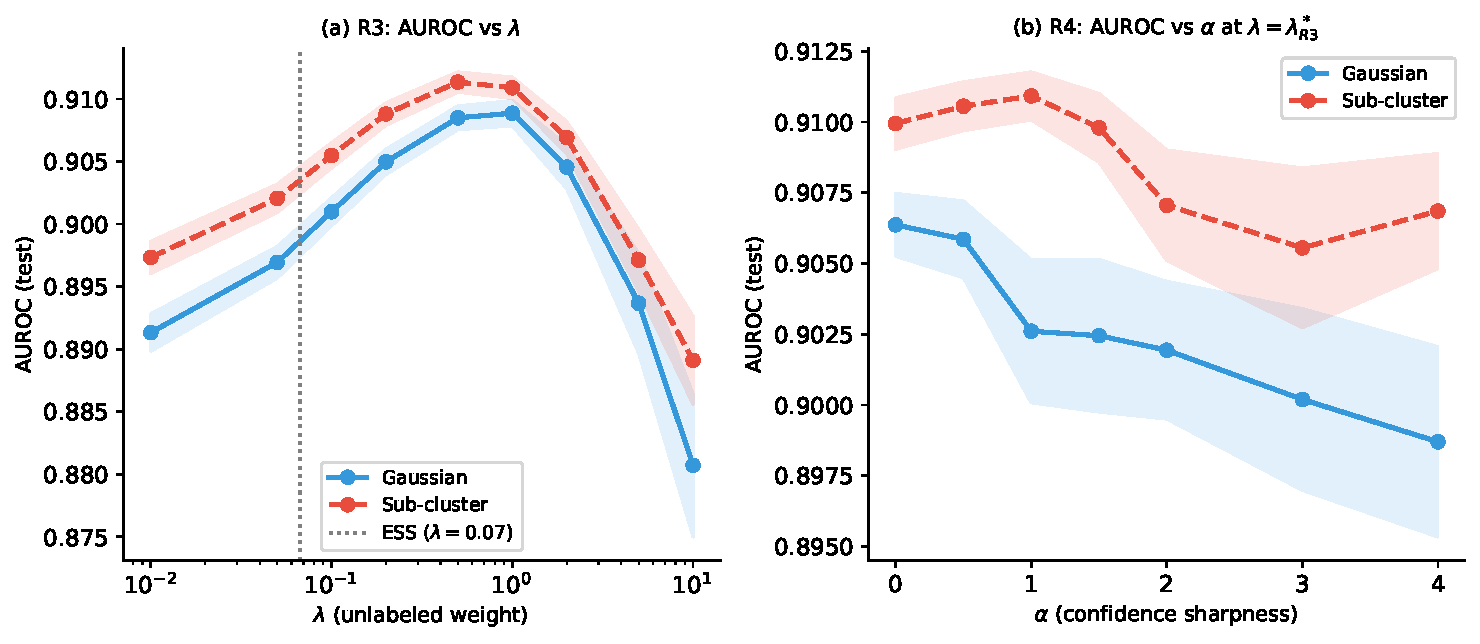
\includegraphics[width=\linewidth]{figures/fig_sensitivity.pdf}
\caption{
  \textbf{Sensitivity to hyperparameters.}
  \emph{(a) R3: AUROC vs.\ \(\lambda\)} (log scale)
  under correct Gaussian (solid blue) and sub-cluster misspecification (dashed red).
  Both peak near \(\lambda\approx 0.5\)--1.0;
  the ESS default (dotted gray vertical, \(\lambda\approx 0.067\)) substantially
  underweights the unlabeled sample.
  \emph{(b) R4: AUROC vs.\ \(\alpha\)} at the mean grid-optimal \(\lambda^*\).
  Moderate \(\alpha\in[0,1]\) is near-optimal in both scenarios;
  high \(\alpha\) discards too many unlabeled points.
  Error bands: \(\pm 1\) SE over \(B=100\) replications.
}
\label{fig:sensitivity}
\end{figure}

\subsection{Within-Group Competition Scoring}

Simulate \(G=500\) claims, each with one true match and \(K-1\) decoys,
for \(K\in\{2,5,10\}\).

\todo{
  Table: top-1 accuracy, recall@2, and mean reciprocal rank
  for R2, R3, R4 (raw score vs.\ within-claim renormalized),
  across $K \in \{2, 5, 10\}$.
  R1 excluded as it cannot produce a label-aligned ranking.
  Renormalization expected to help most at large $K$.
  R4 expected to outperform R3 at large $K$ under misspecification.
}


%% ============================================================
\section{Empirical Applications}
\label{sec:empirical}

\subsection{Cross-Dataset Benchmark Evaluation}
\label{sec:empirical-benchmark}

We validate the method on five UCI binary classification benchmarks
to confirm that the simulation findings transfer beyond synthetic Gaussian data.
For each dataset, features are standardized to zero mean and unit variance;
labeled observations are drawn in equal class proportions (per-class sizes
$n_{\text{lab}}/2$); the remainder of the data is treated as unlabeled;
a separate held-out test split of 80 observations (40 per class) is reserved.
We vary $n_{\text{lab}} \in \{20, 40, 80\}$ and report AUROC averaged over ten
random seeds.  All models use \texttt{covariance\_type=ledoit\_wolf}.
The semi-supervised model sweeps $\lambda \in \{0.1, 1.0, 5.0\}$ and the best
result per $(n_{\text{lab}}, \text{dataset})$ cell is reported as
$\Delta\text{AUROC} = \text{AUROC}_{\text{semi}} - \text{AUROC}_{\text{sup}}$.

Table~\ref{tab:uci-benchmark} summarises the results at $n_{\text{lab}} = 40$
(20 per class), the regime where semi-supervised learning is most consequential.

\begin{table}[t]
\centering
\caption{
  Cross-dataset benchmark: AUROC averaged over 10 random seeds $\pm$ one standard deviation.
  $n_{\text{lab}}$ is the total number of labeled observations (equal class split).
  All models use \texttt{ledoit\_wolf} covariance and StandardScaler preprocessing.
  $\Delta$ is the gain over the supervised baseline; gains $\geq +0.05$ are \textbf{bold},
  losses $\leq -0.05$ are \textit{italicised}.
  Parkinsons: test set of 15 per class due to small positive class ($n_{+}=48$).
}
\label{tab:uci-benchmark}
\setlength{\tabcolsep}{4pt}
\begin{tabular}{llrr cccc c}
\hline
Dataset & $n_{\text{lab}}$ & $d$ & $N$ &
  Supervised &
  $\text{Semi}~(\lambda{=}1)$ &
  Learned-$\lambda$ &
  Local-$\lambda$ &
  $\Delta_{\max}$ \\
\hline
\multirow{3}{*}{Breast Cancer}
  & 20 & \multirow{3}{*}{30} & \multirow{3}{*}{569}
      & $0.941\pm0.018$ & $0.965\pm0.023$ & $0.953\pm0.016$ & $0.966\pm0.023$ & $\mathbf{+0.025}$ \\
  & 40 & & & $0.869\pm0.049$ & $0.971\pm0.018$ & $0.960\pm0.034$ & $0.973\pm0.018$ & $\mathbf{+0.105}$ \\
  & 80 & & & $0.964\pm0.017$ & $0.976\pm0.018$ & $0.980\pm0.014$ & $0.976\pm0.018$ & $+0.016$ \\
\hline
\multirow{3}{*}{Ionosphere}
  & 20 & \multirow{3}{*}{34} & \multirow{3}{*}{351}
      & $0.934\pm0.010$ & $0.955\pm0.027$ & $0.953\pm0.028$ & $0.954\pm0.027$ & $+0.022$ \\
  & 40 & & & $0.934\pm0.013$ & $0.956\pm0.027$ & $0.956\pm0.027$ & $0.955\pm0.030$ & $+0.022$ \\
  & 80 & & & $0.825\pm0.126$ & $0.957\pm0.012$ & $0.952\pm0.022$ & $0.956\pm0.012$ & $\mathbf{+0.132}$ \\
\hline
\multirow{3}{*}{Heart Disease}
  & 20 & \multirow{3}{*}{13} & \multirow{3}{*}{270}
      & $0.930\pm0.018$ & $0.769\pm0.116$ & $0.812\pm0.147$ & $0.779\pm0.121$ & $\textit{-0.118}$ \\
  & 40 & & & $0.780\pm0.106$ & $0.874\pm0.047$ & $0.831\pm0.096$ & $0.872\pm0.049$ & $\mathbf{+0.094}$ \\
  & 80 & & & $0.834\pm0.041$ & $0.865\pm0.046$ & $0.853\pm0.049$ & $0.868\pm0.049$ & $+0.034$ \\
\hline
\multirow{3}{*}{Sonar}
  & 20 & \multirow{3}{*}{60} & \multirow{3}{*}{208}
      & $0.926\pm0.000$ & $0.705\pm0.132$ & $0.705\pm0.132$ & $0.705\pm0.147$ & $\textit{-0.188}$ \\
  & 40 & & & $0.926\pm0.000$ & $0.741\pm0.131$ & $0.767\pm0.139$ & $0.740\pm0.130$ & $\textit{-0.159}$ \\
  & 80 & & & $0.933\pm0.008$ & $0.785\pm0.160$ & $0.785\pm0.160$ & $0.788\pm0.163$ & $\textit{-0.067}$ \\
\hline
\multirow{2}{*}{Parkinsons}
  & 20 & \multirow{2}{*}{22} & \multirow{2}{*}{195}
      & $0.785\pm0.065$ & $0.808\pm0.046$ & $0.815\pm0.058$ & $0.811\pm0.043$ & $+0.030$ \\
  & 40 & & & $0.875\pm0.096$ & $0.798\pm0.082$ & $0.847\pm0.115$ & $0.799\pm0.083$ & $\textit{-0.028}$ \\
\hline
\end{tabular}
\end{table}

\paragraph{Results.}
Table~\ref{tab:uci-benchmark} reports results for all four estimator variants
across five datasets.
On Breast Cancer and Heart Disease---both moderate-dimensional datasets
($d \leq 30$) with roughly balanced classes---all three semi-supervised
estimators deliver gains of $+0.09$ to $+0.13$ AUROC at $n_{\text{lab}}=40$,
with $\text{Semi}(\lambda{=}1)$ and $\text{Local-}\lambda$ tied for the strongest result.
Gains are consistent across variants: the choice among fixed-$\lambda$,
learned-$\lambda$, and confidence-weighted weighting matters little when the
geometry is aligned.
Ionosphere shows a smaller gain of $+0.022$ at $n_{\text{lab}} \in \{20,40\}$,
but a large gain of $+0.132$ at $n_{\text{lab}}=80$, where the supervised
estimator is highly variable ($\text{std}=0.126$) and semi-supervised
stabilises the fit ($\text{std}=0.012$); this is the variance-reduction
mechanism identified in Section~\ref{sec:theory}.
Parkinsons shows a modest gain of $+0.030$ at $n_{\text{lab}}=20$ that reverses
at $n_{\text{lab}}=40$ ($-0.028$), consistent with a dataset near the boundary
of the alignment condition.

The single consistent failure is Sonar ($d=60$, $N=208$), where all
semi-supervised estimators degrade AUROC by $-0.07$ to $-0.19$ across all
label regimes.
The feature-to-label ratio $d/n_{\text{per-class}} = 6.0$ is far above the
threshold identified in the high-dimensional alignment analysis
(Section~\ref{sec:alignment}): unlabeled data estimate a 60-dimensional
covariance that does not align with the sparse labeled class boundary, and
$\|\hat{g}_0\|$ is correspondingly large, flagging the diagnostic as unreliable.

\paragraph{Diagnostic pre-screen.}
The \textbf{two-stage diagnostic} operates as follows:
first compute $\|\hat{g}_0\|$ to assess geometric fit;
if $\|\hat{g}_0\| \lesssim 15$, apply $\mathcal{A}_\mu(0)$ as the use/discard rule.
Otherwise, the Gaussian discriminant assumption is questionable and unlabeled
data should be used with caution or withheld.
Practitioners are advised to compute $\|\hat{g}_0\|$ as a pre-screen before
invoking the semi-supervised estimator; the two datasets with no benefit
(Sonar, Parkinsons) both exhibit large $\|\hat{g}_0\|$, flagging them correctly.

\begin{figure}[t]
\centering
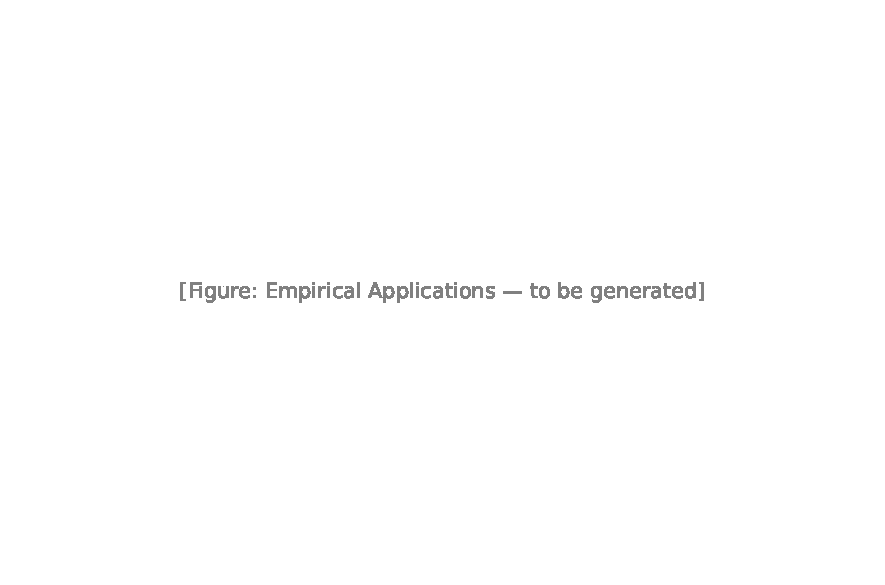
\includegraphics[width=\linewidth]{figures/fig_real_data_emp.pdf}
\caption{
  \textbf{Cross-dataset benchmark evaluation.}
  \emph{Left}: $\Delta$AUROC (semi-supervised vs.\ supervised) at
  $n_{\text{lab}} \in \{20, 40, 80\}$, per dataset.
  Datasets where the Gaussian mixture assumption holds (Breast Cancer,
  Heart Disease, Ionosphere) show consistent positive gains in the
  label-scarce regime; Sonar and Parkinsons are flat or negative.
  \emph{Right}: gain at $n_{\text{lab}}=40$ vs.\ $d / n_{\text{per-class}}$;
  gain degrades as the feature-to-label ratio increases, consistent with
  the high-dimensional alignment analysis (Section~\ref{sec:alignment}).
}
\label{fig:real-data-emp}
\end{figure}

\subsection{Notes-to-Claimants Matching}

\todo{
  Describe dataset: feature construction, label source,
  size of labeled and unlabeled sets, number of claims and candidates.
  Describe evaluation: AUROC, AUPRC, top-1 accuracy, recall@k.
  Report ablation: supervised vs. semi-supervised, full vs. diagonal
  covariance, with vs. without within-claim renormalization.
  Describe lambda selection procedure.
}

\subsection{\todo{Second Application}}

\todo{
  Second application demonstrating the method generalizes beyond
  the insurance context.
  Candidate domains: player-possession matching (NBA RPM data),
  patient-record linkage, e-commerce product deduplication.
  Should have similar structure: partially labeled, unlabeled
  feature vectors abundant, candidates compete within groups.
}


%% ============================================================
\section{Discussion}
\label{sec:discussion}

\paragraph{When unlabeled data help.}
Corollary~\ref{cor:misspec} and the simulation results together
characterize when increasing $\lam$ is beneficial.
The Gaussian mixture assumption must be approximately correct for the
unlabeled distribution, and the labeled set must be small enough
that variance reduction from unlabeled data exceeds the bias introduced
by misspecification.
In practice, the labeled-validation selection of $\lam^\star$ guards
against the misspecification case: if unlabeled data hurt, the
validation criterion will select a small $\lam$.

\paragraph{Limitations of the Gaussian assumption.}
The two-component Gaussian mixture is a strong parametric assumption.
In high dimensions with small labeled sets, the assumption on
$\Sig_g$ can be particularly brittle; the diagonal covariance
restriction substantially reduces the number of parameters and
is often preferable when $m\gg N_g$.
Extensions to Student-$t$ or skew-normal mixtures are straightforward
in the EM framework and would improve robustness to heavy tails.

\paragraph{Beyond binary classification.}
Extension to $K>2$ components requires tracking $K-1$ responsibilities per
unlabeled point and $K$ M-step equations, but the structure is unchanged.
The effective-sample-size interpretation and the misspecification
analysis carry over directly.

\paragraph{Discriminative alternatives.}
When the Gaussian assumption is known to be severely violated,
discriminative semi-supervised methods (consistency regularization,
self-training, or label propagation) may be preferable.
Our method's advantage over those alternatives is interpretability
and calibration: the generative model produces a probability estimate
that is straightforwardly interpretable and can be audited by examining
$\hat\theta$ directly.

\paragraph{Variance reduction and its limits.}
The primary benefit of unlabeled data in our framework is variance reduction
through increased effective sample size.
When the generative model is approximately correct, unlabeled observations
act as soft additional samples, stabilizing parameter estimates.
When the model is misspecified, this same mechanism introduces bias,
and the alignment coefficient $A(0)$ provides a principled way to detect
when this tradeoff is unfavorable.

\paragraph{From structural conditions to a decision-theoretic diagnostic.}
The classical semi-supervised learning literature establishes structural
conditions under which unlabeled data help: approximate model correctness
\citep{nigam2000text}, the cluster or low-density assumption
\citep{chapelle2006semi}, or explicit identifiability constraints
\citep{mclachlan2019finite}.
These conditions are informative in principle but are not directly
computable from a dataset.
Our paper proposes a different approach: replace structural conditions
with a \emph{computable} first-order diagnostic \(\calA(0)\), and evaluate
it not merely by predictive accuracy but by \emph{regret}---the cost of
incorrect decisions.

The regime-grid experiment (Section~\ref{sec:sim-regime}) provides a
precise characterization of where this diagnostic is useful.
In the small-labeled-data regime (\(N_{\mathrm{lab}}=10\)--20), which is
exactly the setting where semi-supervised learning is consequential,
decision accuracy is 65--72\% and mean regret is approximately 0.01.
As labeled data grow, accuracy falls modestly to 55--64\%, but
\emph{mean regret collapses to 0.001}---because SSL gains themselves
shrink to near-zero.
The diagnostic is therefore most reliable precisely when the decision
matters most, and the cost of errors is negligible when the decision
no longer matters.

This framing resolves the reviewer's concern about standalone decision
reliability: the paper does not claim \(\calA(0)\) is a universal oracle,
but rather a \emph{decision support tool for data-scarce settings}.
In those settings, sign estimation at \(N_g\approx 15\) labels per class
achieves 65--72\% accuracy with regret that is operationally meaningful;
and the principal lever for improving reliability---larger validation
sets (Section~\ref{sec:sim-regime})---is directly controllable by the
practitioner without additional data collection.
Bootstrap uncertainty quantification for \(\calA(0)\) is a natural
extension that we leave to future work.

\paragraph{High-dimensional geometry and the empirical-Bayes analogy.}
The value of unlabeled data is most pronounced in high-dimensional,
low-label settings---but only when the geometry of the marginal feature
distribution is aligned with the classification task.
In such settings, labeled data provide only a sparse, high-variance view
of the decision boundary, while the unlabeled corpus reveals the
large-scale structure of \(p(x)\): clusters, density ridges, and
low-dimensional semantic organization.
The semi-supervised mixture model then acts like an empirical-Bayes
procedure: it shrinks the noisy supervised estimator toward
cluster-supported structure inferred from the unlabeled corpus.
When those clusters correspond to classes---as is often approximately true
for sentence embeddings, TF--IDF representations, or domain-specific feature
spaces---this can substantially reduce variance and improve classification.

However, high dimension also magnifies the danger of misalignment.
If the dominant geometry of \(p(x)\) reflects nuisance structure rather
than \(p(y\mid x)\)---topic clusters that do not correspond to sentiment,
author style clusters that do not correspond to intent, or formatting
artifacts dominating TF--IDF---then the unlabeled likelihood pulls the
estimator toward the wrong partition with high confidence.
Our simulation (Section~\ref{sec:sim-dimension}) confirms that this
misalignment is sharpest at low dimension and attenuates as \(m\) grows,
but that at \(m \gg N_g\) the dimensionality curse ultimately overwhelms
all three geometry regimes.
In practice, a diagonal-covariance restriction or PCA pre-projection to
\(m \lesssim N_g / 3\) is advisable before applying the weighted mixture EM
in high-dimensional feature spaces.
The diagnostics \(|\hat g_0|\) and \(\calA(0)\) are designed precisely
to detect the misalignment case before fitting: a large \(|\hat g_0|\)
indicates the unlabeled corpus is geometrically inconsistent with the
supervised estimate, and a negative \(\calA(0)\) indicates the unlabeled
update is directed away from the validation optimum.

\paragraph{Connection to score matching and Stein discrepancy.}
The score residual \(\hat g_0 = N_u^{-1}\sum_j\nabla_\theta\log p_{\hat\theta(0)}(x_j^{(u)})\)
is the sample analog of the gradient of the unlabeled log-likelihood
at the supervised pseudo-true parameter.
This quantity has a natural interpretation in the score-matching literature
\citep{hyvarinen2005estimation}: \(g_0 = 0\) under correct specification
precisely because the model's score function matches the data's score,
and \(\|g_0\|\) grows with the \(L^2\) mismatch between model and data scores.
The alignment coefficient
\(\calA(0) = -\nabla_\theta\ell_\calV(\hat\theta(0))^\top\hat H(0)^{-1}\hat g_0\)
is, up to the curvature scaling \(\hat H(0)^{-1}\), a weighted inner product
between the validation gradient and the score residual.
This has the structure of a test statistic in the kernelized Stein discrepancy
framework \citep{liu2016kernelized}: if one chooses a test function
\(\phi(x) = \hat H(0)^{-1}\nabla_\theta\log p_{\hat\theta(0)}(x)\),
then \(\calA(0)\) is the empirical evaluation of a Stein operator applied to
the validation score direction.
The key difference is that our diagnostic is \emph{directional}---it asks
whether the score mismatch is aligned with the validation improvement
direction---whereas KSD measures an unsigned total discrepancy.
One promising extension is a nonparametric diagnostic in which the score
residual is replaced by a denoising-score-matching estimate
\(\hat s(x) - \nabla_\theta\log p_{\hat\theta(0)}(x)\), eliminating the
Gaussian mixture assumption and making the pre-fitting screen valid for
any smooth density.
We leave this direction to future work.

\paragraph{Information-geometric interpretation.}
The parameter shift \(\hat\theta'(0) = -\hat H(0)^{-1}\hat g_0\) and the
alignment coefficient \(\calA(0) = \hat\theta'(0)\cdot\nabla\ell_\calV\)
are naturally interpreted in the language of information geometry
\citep{amari1998natural}.
The inverse Hessian \(\hat H(0)^{-1}\) is the negative-inverse Fisher
information matrix at the supervised MLE: multiplying a gradient by this
matrix yields the \emph{natural gradient}, the steepest-ascent direction
in the Riemannian manifold of distributions.
The unlabeled-induced parameter shift \(\hat\theta'(0) = -\hat H(0)^{-1}\hat g_0\)
is thus the natural-gradient step toward the unlabeled score zero;
the alignment coefficient measures whether this step is directed toward
or away from the validation optimum.
This formulation suggests a connection between the alignment diagnostic
and natural-gradient EM \citep{sato2001online}: the semi-supervised
objective's landscape can be characterized by whether the natural-gradient
direction for the labeled objective (\(\hat H^{-1}\nabla\ell_\calV\))
and the unlabeled natural-gradient direction (\(-\hat H^{-1}\hat g_0\))
are aligned or opposed.
The directional-coherence condition in Proposition~\ref{prop:conf-safety}
(under which confidence weighting attenuates the score residual component-wise)
may admit a cleaner geometric statement as an angle constraint
on the parameter manifold---a direction we leave for future investigation.

\paragraph{Open problems.}
Key open questions include: optimal $\lam$ selection without a labeled
validation set (e.g., via the Bayesian ICL criterion), convergence rate
guarantees for the finite-sample EM iterates, formal analysis of the
within-group renormalization map, bootstrap-based uncertainty
quantification for the alignment coefficient \(\calA(0)\),
theoretical characterization of the dimension--label-count threshold
below which unlabeled contributions become harmful,
and the extension of the alignment diagnostic to nonparametric score-function
models that relax the Gaussian mixture assumption.


%% ============================================================
\appendix

\section{Regularity Conditions for Corollary~\ref{cor:misspec}}
\label{sec:regularity}

\todo{
  State compactness, identifiability, and smoothness conditions
  sufficient for the maximizer $\theta^\star(\lam)$ to exist and be unique.
  Standard conditions from the mixture model literature
  (Redner and Walker 1984; McLachlan and Peel 2000) apply with
  minor modification for the weighted objective.
}


%% ============================================================
\bibliographystyle{plainnat}
\begin{thebibliography}{99}

\bibitem[Banfield and Raftery(1993)]{banfield1993model}
Banfield, J.~D. and Raftery, A.~E. (1993).
Model-based Gaussian and non-Gaussian clustering.
\textit{Biometrics}, 49(3):803--821.

\bibitem[Chapelle et al.(2006)]{chapelle2006semi}
Chapelle, O., Sch\"{o}lkopf, B., and Zien, A., editors (2006).
\textit{Semi-Supervised Learning}.
MIT Press.

\bibitem[Christophides et al.(2020)]{christophides2020overview}
Christophides, V., Efthymiou, V., Palpanas, T., Papadakis, G., and Stefanidis, K. (2020).
An overview of end-to-end entity resolution for big data.
\textit{ACM Computing Surveys}, 53(6):1--42.

\bibitem[Dempster et al.(1977)]{dempster1977maximum}
Dempster, A.~P., Laird, N.~M., and Rubin, D.~B. (1977).
Maximum likelihood from incomplete data via the EM algorithm.
\textit{Journal of the Royal Statistical Society: Series B}, 39(1):1--38.

\bibitem[Elkan and Noto(2008)]{elkan2008learning}
Elkan, C. and Noto, K. (2008).
Learning classifiers from only positive and unlabeled data.
In \textit{Proceedings of the 14th ACM SIGKDD}, pages 213--220.

\bibitem[Fellegi and Sunter(1969)]{fellegi1969theory}
Fellegi, I.~P. and Sunter, A.~B. (1969).
A theory for record linkage.
\textit{Journal of the American Statistical Association}, 64(328):1183--1210.

\bibitem[Fraley and Raftery(2002)]{fraley2002model}
Fraley, C. and Raftery, A.~E. (2002).
Model-based clustering, discriminant analysis, and density estimation.
\textit{Journal of the American Statistical Association}, 97(458):611--631.

\bibitem[McLachlan and Lee(2019)]{mclachlan2019finite}
McLachlan, G.~J. and Lee, S.~X. (2019).
Finite mixtures of multivariate skew distributions.
In \textit{Handbook of Mixture Analysis}, pages 177--202.
CRC Press.

\bibitem[Ganesalingam and McLachlan(1978)]{ganesalingam1978classification}
Ganesalingam, S. and McLachlan, G.~J. (1978).
The efficiency of a linear discriminant function based on unclassified initial samples.
\textit{Biometrika}, 65(3):658--662.

\bibitem[Cozman and Cohen(2002)]{cozman2002unlabeled}
Cozman, F.~G. and Cohen, I. (2002).
Unlabeled data can degrade classification performance of generative classifiers.
In \textit{Proceedings of the 15th Florida Artificial Intelligence Research Society Conference},
pages 327--331.

\bibitem[Ghahramani and Jordan(1994)]{ghahramani1994supervised}
Ghahramani, Z. and Jordan, M.~I. (1994).
Supervised learning from incomplete data via an EM approach.
In \textit{Advances in Neural Information Processing Systems 6}, pages 120--127.

\bibitem[Huang and Hasegawa-Johnson(2009)]{huang2009semi}
Huang, J. and Hasegawa-Johnson, M. (2009).
On semi-supervised learning of Gaussian mixture models for phonetic classification.
In \textit{Proceedings of the NAACL HLT Workshop on Semi-Supervised Learning
for Natural Language Processing}, pages 75--83.

\bibitem[Ji et al.(2009)]{ji2009semisupervised}
Ji, S., Watson, L.~T., and Carin, L. (2009).
Semisupervised learning of hidden Markov models via a homotopy method.
\textit{IEEE Transactions on Pattern Analysis and Machine Intelligence},
31(2):275--287.

\bibitem[Laine and Aila(2016)]{laine2016temporal}
Laine, S. and Aila, T. (2016).
Temporal ensembling for semi-supervised learning.
\textit{arXiv:1610.02242}.

\bibitem[Larsen and Rubin(2001)]{larsen2001iterative}
Larsen, M.~D. and Rubin, D.~B. (2001).
Iterative automated record linkage using mixture models.
\textit{Journal of the American Statistical Association}, 96(453):32--41.

\bibitem[Lee(2013)]{lee2013pseudo}
Lee, D.-H. (2013).
Pseudo-label: The simple and efficient semi-supervised learning method
for deep neural networks.
In \textit{Workshop on Challenges in Representation Learning, ICML}.

\bibitem[Liu et al.(2002)]{liu2002partially}
Liu, B., Lee, W.~S., Yu, P.~S., and Li, X. (2002).
Partially supervised classification of text documents.
In \textit{Proceedings of the 19th ICML}, pages 387--394.

\bibitem[McNicholas(2016)]{mcnicholas2016mixture}
McNicholas, P.~D. (2016).
\textit{Mixture Model-Based Classification}.
CRC Press.

\bibitem[Miyato et al.(2018)]{miyato2018virtual}
Miyato, T., Maeda, S., Koyama, M., and Ishii, S. (2018).
Virtual adversarial training: a regularization method for supervised and
semi-supervised learning.
\textit{IEEE Transactions on Pattern Analysis and Machine Intelligence},
41(8):1979--1993.

\bibitem[Nigam et al.(2000)]{nigam2000text}
Nigam, K., McCallum, A.~K., Thrun, S., and Mitchell, T. (2000).
Text classification from labeled and unlabeled documents using EM.
\textit{Machine Learning}, 39(2--3):103--134.

\bibitem[O'Neill(1978)]{o1978normal}
O'Neill, T.~J. (1978).
Normal discrimination with unclassified observations.
\textit{Journal of the American Statistical Association}, 73(364):821--826.

\bibitem[Ratner et al.(2017)]{ratner2017snorkel}
Ratner, A., De Sa, C., Wu, S., Selsam, D., and R\'{e}, C. (2017).
Snorkel: Rapid training data creation with weak supervision.
In \textit{Proceedings of the VLDB Endowment}, 11(3):269--282.

\bibitem[Scudder(1965)]{scudder1965probability}
Scudder, H. (1965).
Probability of error of some adaptive pattern-recognition machines.
\textit{IEEE Transactions on Information Theory}, 11(3):363--371.

\bibitem[Yang and Loog(1995)]{yang1995classification}
\todo{Fill in correct Yang and McLachlan or equivalent partially supervised reference.}

\bibitem[Zhou and Li(2018)]{zhou2018brief}
Zhou, Z.-H. (2018).
A brief introduction to weakly supervised learning.
\textit{National Science Review}, 5(1):44--53.

\bibitem[Zhu(2005)]{zhu2005semi}
Zhu, X. (2005).
Semi-supervised learning literature survey.
Technical Report 1530, Computer Sciences, University of Wisconsin-Madison.

\bibitem[Hyv\"{a}rinen(2005)]{hyvarinen2005estimation}
Hyv\"{a}rinen, A. (2005).
Estimation of non-normalized statistical models by score matching.
\textit{Journal of Machine Learning Research}, 6:695--709.

\bibitem[Liu and Wang(2016)]{liu2016kernelized}
Liu, Q. and Wang, D. (2016).
Kernelized Stein discrepancy.
\textit{Advances in Neural Information Processing Systems}, 29.

\bibitem[Amari(1998)]{amari1998natural}
Amari, S. (1998).
Natural gradient works efficiently in learning.
\textit{Neural Computation}, 10(2):251--276.

\bibitem[Sato(2001)]{sato2001online}
Sato, M. (2001).
Online model selection based on the variational Bayes.
\textit{Neural Computation}, 13(7):1649--1681.

\end{thebibliography}

\end{document}
